% Options for packages loaded elsewhere
\PassOptionsToPackage{unicode}{hyperref}
\PassOptionsToPackage{hyphens}{url}
\PassOptionsToPackage{dvipsnames,svgnames,x11names}{xcolor}
%
\documentclass[
]{article}
\usepackage{amsmath,amssymb}
\usepackage{lmodern}
\usepackage{iftex}
\ifPDFTeX
  \usepackage[T1]{fontenc}
  \usepackage[utf8]{inputenc}
  \usepackage{textcomp} % provide euro and other symbols
\else % if luatex or xetex
  \usepackage{unicode-math}
  \defaultfontfeatures{Scale=MatchLowercase}
  \defaultfontfeatures[\rmfamily]{Ligatures=TeX,Scale=1}
\fi
% Use upquote if available, for straight quotes in verbatim environments
\IfFileExists{upquote.sty}{\usepackage{upquote}}{}
\IfFileExists{microtype.sty}{% use microtype if available
  \usepackage[]{microtype}
  \UseMicrotypeSet[protrusion]{basicmath} % disable protrusion for tt fonts
}{}
\makeatletter
\@ifundefined{KOMAClassName}{% if non-KOMA class
  \IfFileExists{parskip.sty}{%
    \usepackage{parskip}
  }{% else
    \setlength{\parindent}{0pt}
    \setlength{\parskip}{6pt plus 2pt minus 1pt}}
}{% if KOMA class
  \KOMAoptions{parskip=half}}
\makeatother
\usepackage{xcolor}
\usepackage[margin=1in]{geometry}
\usepackage{longtable,booktabs,array}
\usepackage{calc} % for calculating minipage widths
% Correct order of tables after \paragraph or \subparagraph
\usepackage{etoolbox}
\makeatletter
\patchcmd\longtable{\par}{\if@noskipsec\mbox{}\fi\par}{}{}
\makeatother
% Allow footnotes in longtable head/foot
\IfFileExists{footnotehyper.sty}{\usepackage{footnotehyper}}{\usepackage{footnote}}
\makesavenoteenv{longtable}
\usepackage{graphicx}
\makeatletter
\def\maxwidth{\ifdim\Gin@nat@width>\linewidth\linewidth\else\Gin@nat@width\fi}
\def\maxheight{\ifdim\Gin@nat@height>\textheight\textheight\else\Gin@nat@height\fi}
\makeatother
% Scale images if necessary, so that they will not overflow the page
% margins by default, and it is still possible to overwrite the defaults
% using explicit options in \includegraphics[width, height, ...]{}
\setkeys{Gin}{width=\maxwidth,height=\maxheight,keepaspectratio}
% Set default figure placement to htbp
\makeatletter
\def\fps@figure{htbp}
\makeatother
\setlength{\emergencystretch}{3em} % prevent overfull lines
\providecommand{\tightlist}{%
  \setlength{\itemsep}{0pt}\setlength{\parskip}{0pt}}
\setcounter{secnumdepth}{5}
\usepackage{float}
\floatplacement{Figure}{H}
\usepackage{flafter}
\ifLuaTeX
  \usepackage{selnolig}  % disable illegal ligatures
\fi
\IfFileExists{bookmark.sty}{\usepackage{bookmark}}{\usepackage{hyperref}}
\IfFileExists{xurl.sty}{\usepackage{xurl}}{} % add URL line breaks if available
\urlstyle{same} % disable monospaced font for URLs
\hypersetup{
  pdftitle={Vancouver Housing Report},
  pdfauthor={Pascal Schmidt},
  colorlinks=true,
  linkcolor={Maroon},
  filecolor={Maroon},
  citecolor={Blue},
  urlcolor={blue},
  pdfcreator={LaTeX via pandoc}}

\title{Vancouver Housing Report}
\author{Pascal Schmidt}
\date{2023-03-10}

\begin{document}
\maketitle

{
\hypersetup{linkcolor=}
\setcounter{tocdepth}{2}
\tableofcontents
}
\newpage

\hypertarget{introduction-and-research-question}{%
\section{Introduction and Research
Question}\label{introduction-and-research-question}}

Housing is an area of life that is affecting everyone. With an
ever-changing economy and increasing interest rates, it is difficult to
price properties accurately. Therefore, I was interested in analyzing
the Vancouver real estate market and predicting the listing price of a
property. This lets interested buyers and sellers in the Vancouver
market know what they can roughly expect a home will cost when trying to
buy or sell a property. To answer this research question I scraped data
from real estate websites and feature engineered variables with the
Google Maps API and publicly available data sets. I then used a random
forest model and a gradient-boosted decision tree to predict the listing
price of a home.

\hypertarget{data-acquisition}{%
\section{Data Acquisition}\label{data-acquisition}}

\hypertarget{introduction}{%
\subsection{Introduction}\label{introduction}}

It is important to have the right predictor variables that explain the
variation in property prices well. Therefore, I looked for a variety of
websites that allowed me to scrape their data. One reason to scrape from
multiple websites was to increase the sample size of my data and another
reason was to reduce the selection bias of home prices. This eliminates
the chance of scraping homes from websites that only list, for example,
luxury homes or only homes from certain neighborhoods in Vancouver.
Also, maybe only certain agents list properties on certain websites and
there is a variation in how much a property costs, based on a property
agent.

On top of scraping data from the web, I also augmented my existing data
set with publicly available data from the City of Vancouver, the police
department, and the public transit website from Vancouver. This allowed
me to get information about public schools, parks, restaurants and bars,
crime rates, and bus and train stations. In addition to these data
sources, I also used the Google Maps API to get latitude and longitude
values for all the properties I scraped, by providing the API with the
scraped property addresses. To accomplish this I created API credentials
on the \href{https://cloud.google.com/products}{Google Cloud Platform}
to access the geocoding functionality. I then used the
\texttt{googleway} package to send addresses to the API and got back
latitude and longitude values for the properties I scraped.

\hypertarget{web-scraping-details}{%
\subsection{Web Scraping Details}\label{web-scraping-details}}

In total, I scraped rental prices and property prices from six different
real estate websites. Table 1 shows the websites. Point 2 Homes, Remax,
Rew, and Zolo provided data for property prices and Craigslist and
Live.Rent provided rentals rates.

\begin{longtable}[]{@{}
  >{\raggedright\arraybackslash}p{(\columnwidth - 2\tabcolsep) * \real{0.4780}}
  >{\raggedright\arraybackslash}p{(\columnwidth - 2\tabcolsep) * \real{0.5220}}@{}}
\caption{Scraped Websites}\tabularnewline
\toprule()
\begin{minipage}[b]{\linewidth}\raggedright
Property Listing Websites
\end{minipage} & \begin{minipage}[b]{\linewidth}\raggedright
Rental Listing Websites
\end{minipage} \\
\midrule()
\endfirsthead
\toprule()
\begin{minipage}[b]{\linewidth}\raggedright
Property Listing Websites
\end{minipage} & \begin{minipage}[b]{\linewidth}\raggedright
Rental Listing Websites
\end{minipage} \\
\midrule()
\endhead
\href{https://www.point2homes.com/CA/Real-Estate-Listings/BC/Vancouver.html}{Point
2 Homes} &
\href{https://vancouver.craigslist.org/search/apa?query=Vancouver\#search=1~gallery~0~0}{Craigslist} \\
\href{https://www.remax.ca/bc/vancouver-real-estate?pageNumber=1}{Remax}
& \href{https://liv.rent/rental-listings/city/vancouver}{Liv.rent} \\
\href{https://www.rew.ca/properties/areas/vancouver-bc}{Rew} & \\
\href{https://www.zolo.ca/vancouver-real-estate}{Zolo} & \\
\bottomrule()
\end{longtable}

A big challenge of scraping multiple data sources was to obtain common
predictors from all websites. Point 2 home, Rew, and Zolo had data about
lot sizes but Remax did not. So I decided to exclude properties of type
single family home from Remax and only included apartments and condos
that had no lot size. Another trade-off I made when combining different
data sources was to exclude the year a house was built. Some of the
websites I scraped did not include this information while others did.
Ultimately, I decided to include more observations in my sample from
different data sources rather than deleting observations that did not
have the predictor for when a property was built.

For dynamic websites, I used the \texttt{RSelenium} package in
combination with a Docker container to scrape real estate listings. For
static websites, I used the \texttt{rvest} package.

For each website, I created two web scraping functions. One function
scrapes all the links that point to the individual property website and
a second one visits the scraped links and scrapes all the necessary
information for a property. I started scraping websites in late January
and periodically scraped data until late March. When I was re-running
the web scraping functions I excluded links that were scraped in the
past.

Table 2 shows all the variables scraped from the websites that are
listed in Table 1.

\begin{longtable}[]{@{}l@{}}
\caption{Variables Scraped From Websites}\tabularnewline
\toprule()
Variables From Web Scraping \\
\midrule()
\endfirsthead
\toprule()
Variables From Web Scraping \\
\midrule()
\endhead
Price \\
\# of Bedrooms \\
\# of Bathrooms \\
\# of Square Feet \\
Lot Size in Square Feet \\
Address \\
Type of Home \\
\bottomrule()
\end{longtable}

\hypertarget{public-places-details}{%
\subsection{Public Places Details}\label{public-places-details}}

In addition to the variables obtained from web scraping, I also visited
the City of Vancouver website to find data sets and variables that are
useful to predict the price of a property. In particular, I acquired
data sets about
\href{https://opendata.vancouver.ca/explore/dataset/schools/table/}{schools},
\href{https://opendata.vancouver.ca/explore/dataset/parks-polygon-representation/table/}{parks},
\href{https://opendata.vancouver.ca/explore/dataset/storefronts-inventory/table/}{places}
such as grocery stores, restaurants, coffee shops, and public service
places. Each of these data sets had latitude and longitude values
included.

I also was interested in finding out about public transit stations. I
found information about bus stops and sky train stations on the official
\href{(https://www.translink.ca/about-us/doing-business-with-translink/app-developer-resources/gtfs/gtfs-data)}{Translink}
website where I used the \texttt{stops.txt} file for information about
bus stops and sky train stops in Vancouver. The stops had latitude and
longitude associated with them.

For the schools, parks, and transit stations, I calculated the shortest
distance from a property to these places. For restaurants, coffee shops,
convenience stores, and commercial services, I calculated how many of
these places are in a 500m radius around the home. To calculate the
distances, I connected to the Google Maps API and used the address I
scraped to get back latitude and longitude values. I used the
coordinates from the property and also the coordinates from the public
places to calculate the distances. I also used the latitude and
longitude values from the Google Maps API as predictors in my model.

In addition to the public places, I also visited the website for the
\href{https://geodash.vpd.ca/opendata/}{Vancouver police department} and
downloaded crime rates by neighborhood and crime type. Unfortunately,
due to privacy reasons, no latitude and longitude values were provided.
However, addresses for intersections and blocks were provided. I added
latitude and longitude values with the help of the Google Maps API and
then summarized the number of crimes by neighborhood and crime type and
added it to the existing data frame.

I was also interested in finding out the neighborhood of a home. Some of
the websites I scraped did not list the neighborhood of a property.
Therefore, I downloaded a shape file from the City of Vancouver
\href{https://opendata.vancouver.ca/explore/dataset/local-area-boundary/table/?disjunctive.name}{open
data portal} that includes polygon data about all neighborhoods in
Vancouver. I then calculated if a coordinate falls within a polygon and
added a neighborhood column to my data set.

\hypertarget{sample-size}{%
\subsection{Sample Size}\label{sample-size}}

In total, I scraped around \textasciitilde20,000 observations from real
estate websites. Around 1/3 of the observations come from rentals and
2/3 of observations come from property prices. The information I was
scraping from the websites were the address of the home, number of
bathrooms, number of bedrooms, number of square feet, the type of the
home (condo, duplex, single-family home, etc), the lot size, and the
price of the home.

Figure 1 shows a flow chart of the sample size. I am starting with
20,000 observations which are the raw data. After collecting latitude
and longitude values with the help of the Google Maps API there are
around 18,200 observations left. This is either because the web scraper
failed to scrape the address properly or because Google gave back an
address that is not exact. With each API call, Google sends back the
location type. If the location type was not \texttt{ROOFTOP} or
\texttt{APPROXIMATE}, observations were deleted.

Sometimes, web scrapers failed to scrape the necessary predictors,
listed in Table 1, from the websites or some websites had missing
information. This is particularly true for a website such as craigslist
where users input the data and often leave out information. Therefore,
all observations that had one or more predictors missing from Table 1
were deleted. This resulted in 14,000 observations.

Next, only observations from Vancouver neighborhoods were considered.
Originally, also properties in the Greater Vancouver area were
considered such as Burnaby, Richmond, Surrey, and North Vancouver.
However, due to more data collection efforts such as public places and
the increase in API calls, which is costly, I decided to only focus on
the Vancouver neighborhoods. After intersecting the latitude and
longitude data with the polygon regions obtained from the City of
Vancouver and excluding properties worth \$10 million or more, only
around 7,000 observations were left. I excluded properties worth \$10
Million or more because there were too few observations in that price
range. The Appendix Table 11 shows all the neighborhoods that were
considered and Figure 21 shows how many properties are present in each
neighborhood.

\begin{figure}
\centering
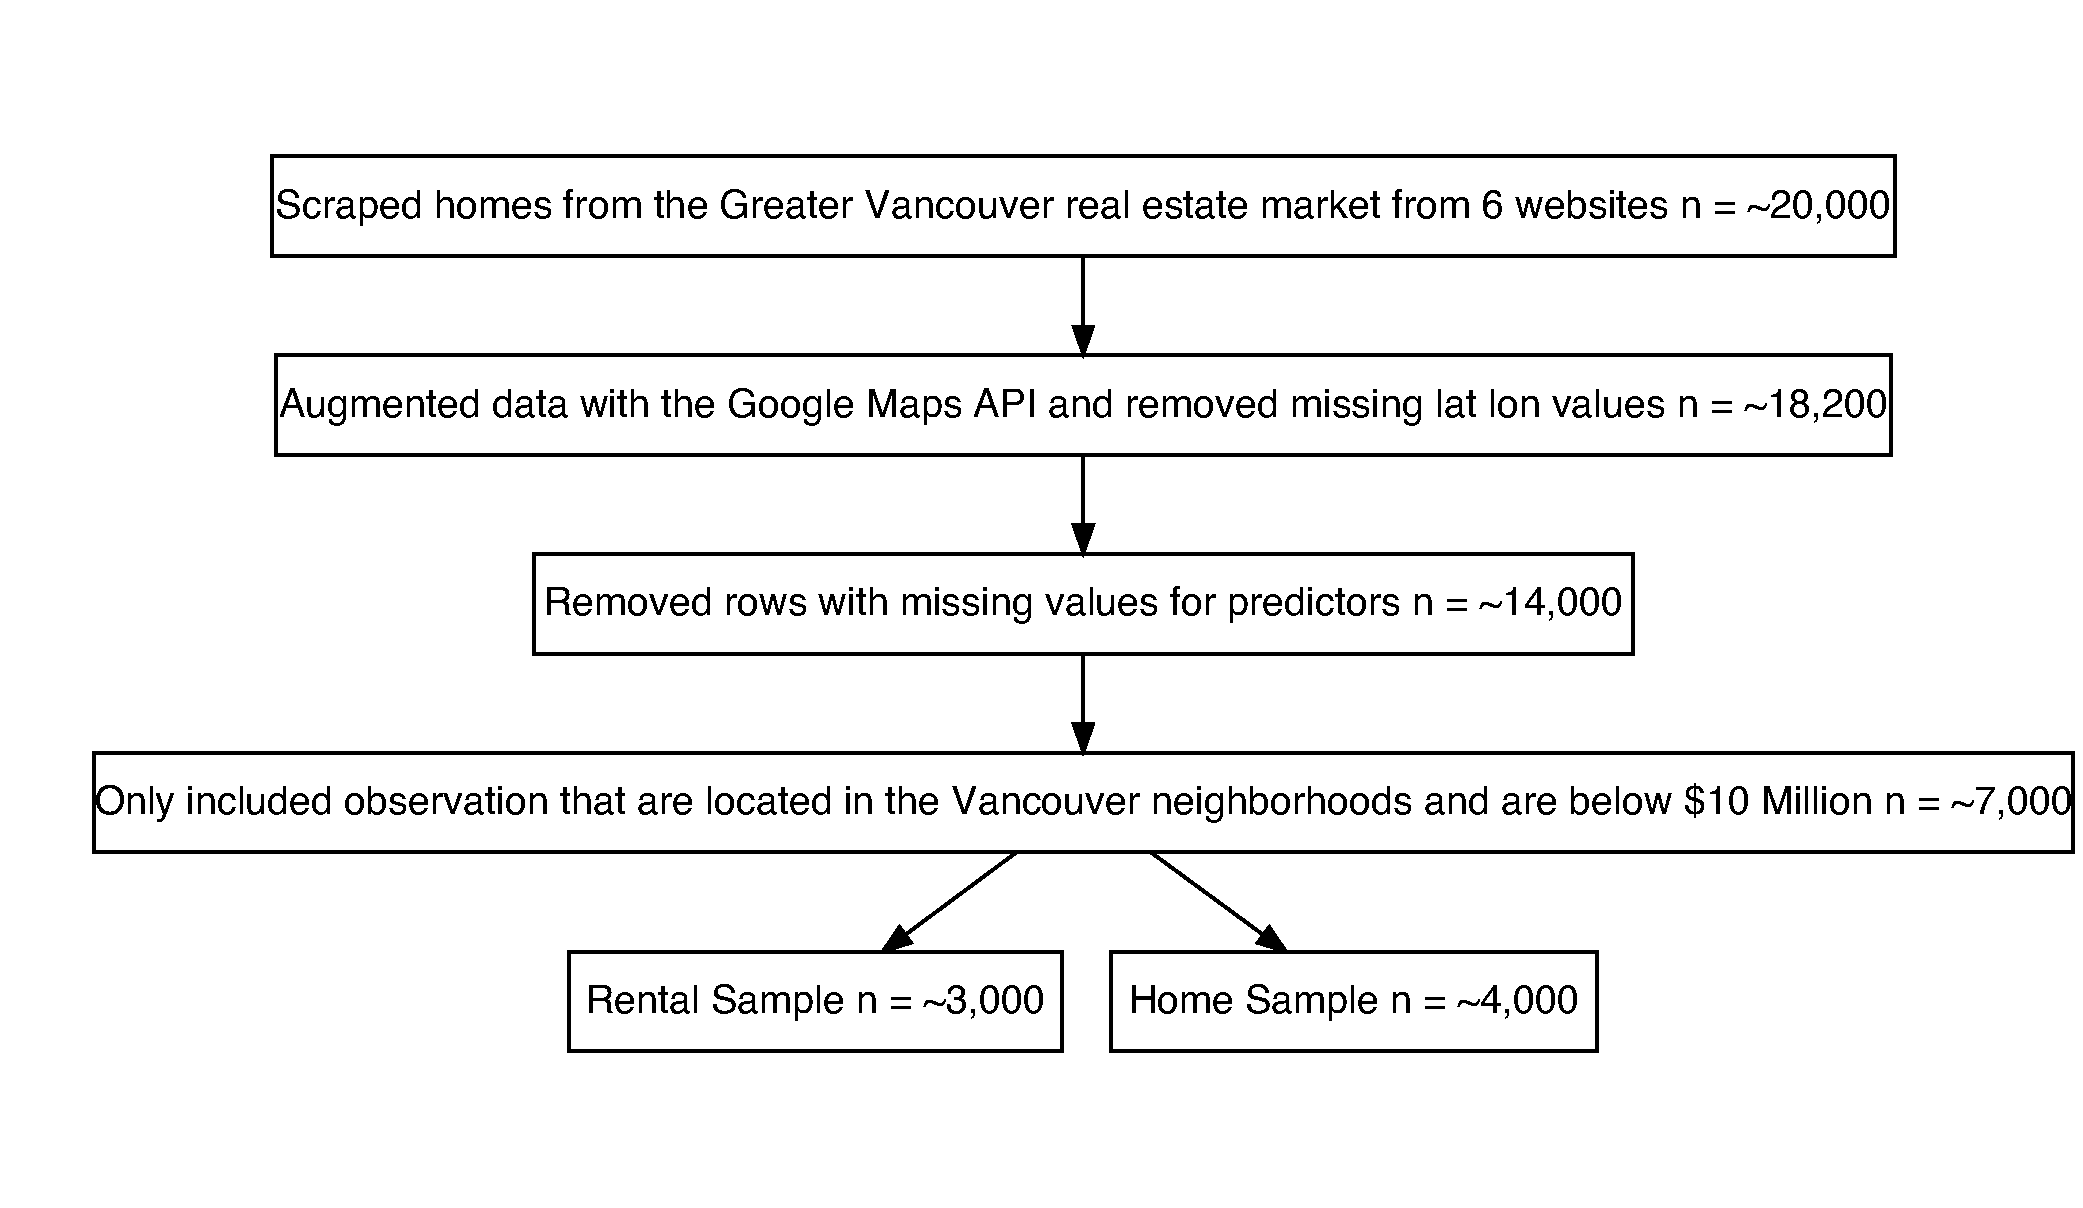
\includegraphics{final_report_files/figure-latex/sample-size-1.pdf}
\caption{Sample Size Flow Chart}
\end{figure}

\hypertarget{data-storage}{%
\subsection{Data Storage}\label{data-storage}}

Figure 2 shows the data storage process. Because I was web scraping data
periodically I created one parquet file for each website and day when I
was scraping. This resulted in around 5-6 parquet files for each website
that included the raw data from late January to late March. After I
scraped data from the websites listed in Table 1, I did some
pre-cleaning steps that were unique to each scraped website. Such
cleaning steps involved coercing character strings into numeric data
types, lumping levels together for categorical predictors and merging
columns when the same information was distributed across multiple
columns. On top of that I also removed unnecessary variables for example
when a property was built, the property description, home features, and
if pets were allowed or not.

I used one folder for every website I scraped. I created parquet files
every time I was scraping data and the file was named according to the
date I obtained the data. In addition to the cleaning steps, I also
feature engineered latitude and longitude values for each property.
After the cleaning steps and data augmentation step I created a new
folder and split all the data into separate parquet files by the date it
was collected.

Figure 22 in the Appendix explains what R functions and scripts were
used from scraping the data to creating the final data set.

\begin{figure}
\centering
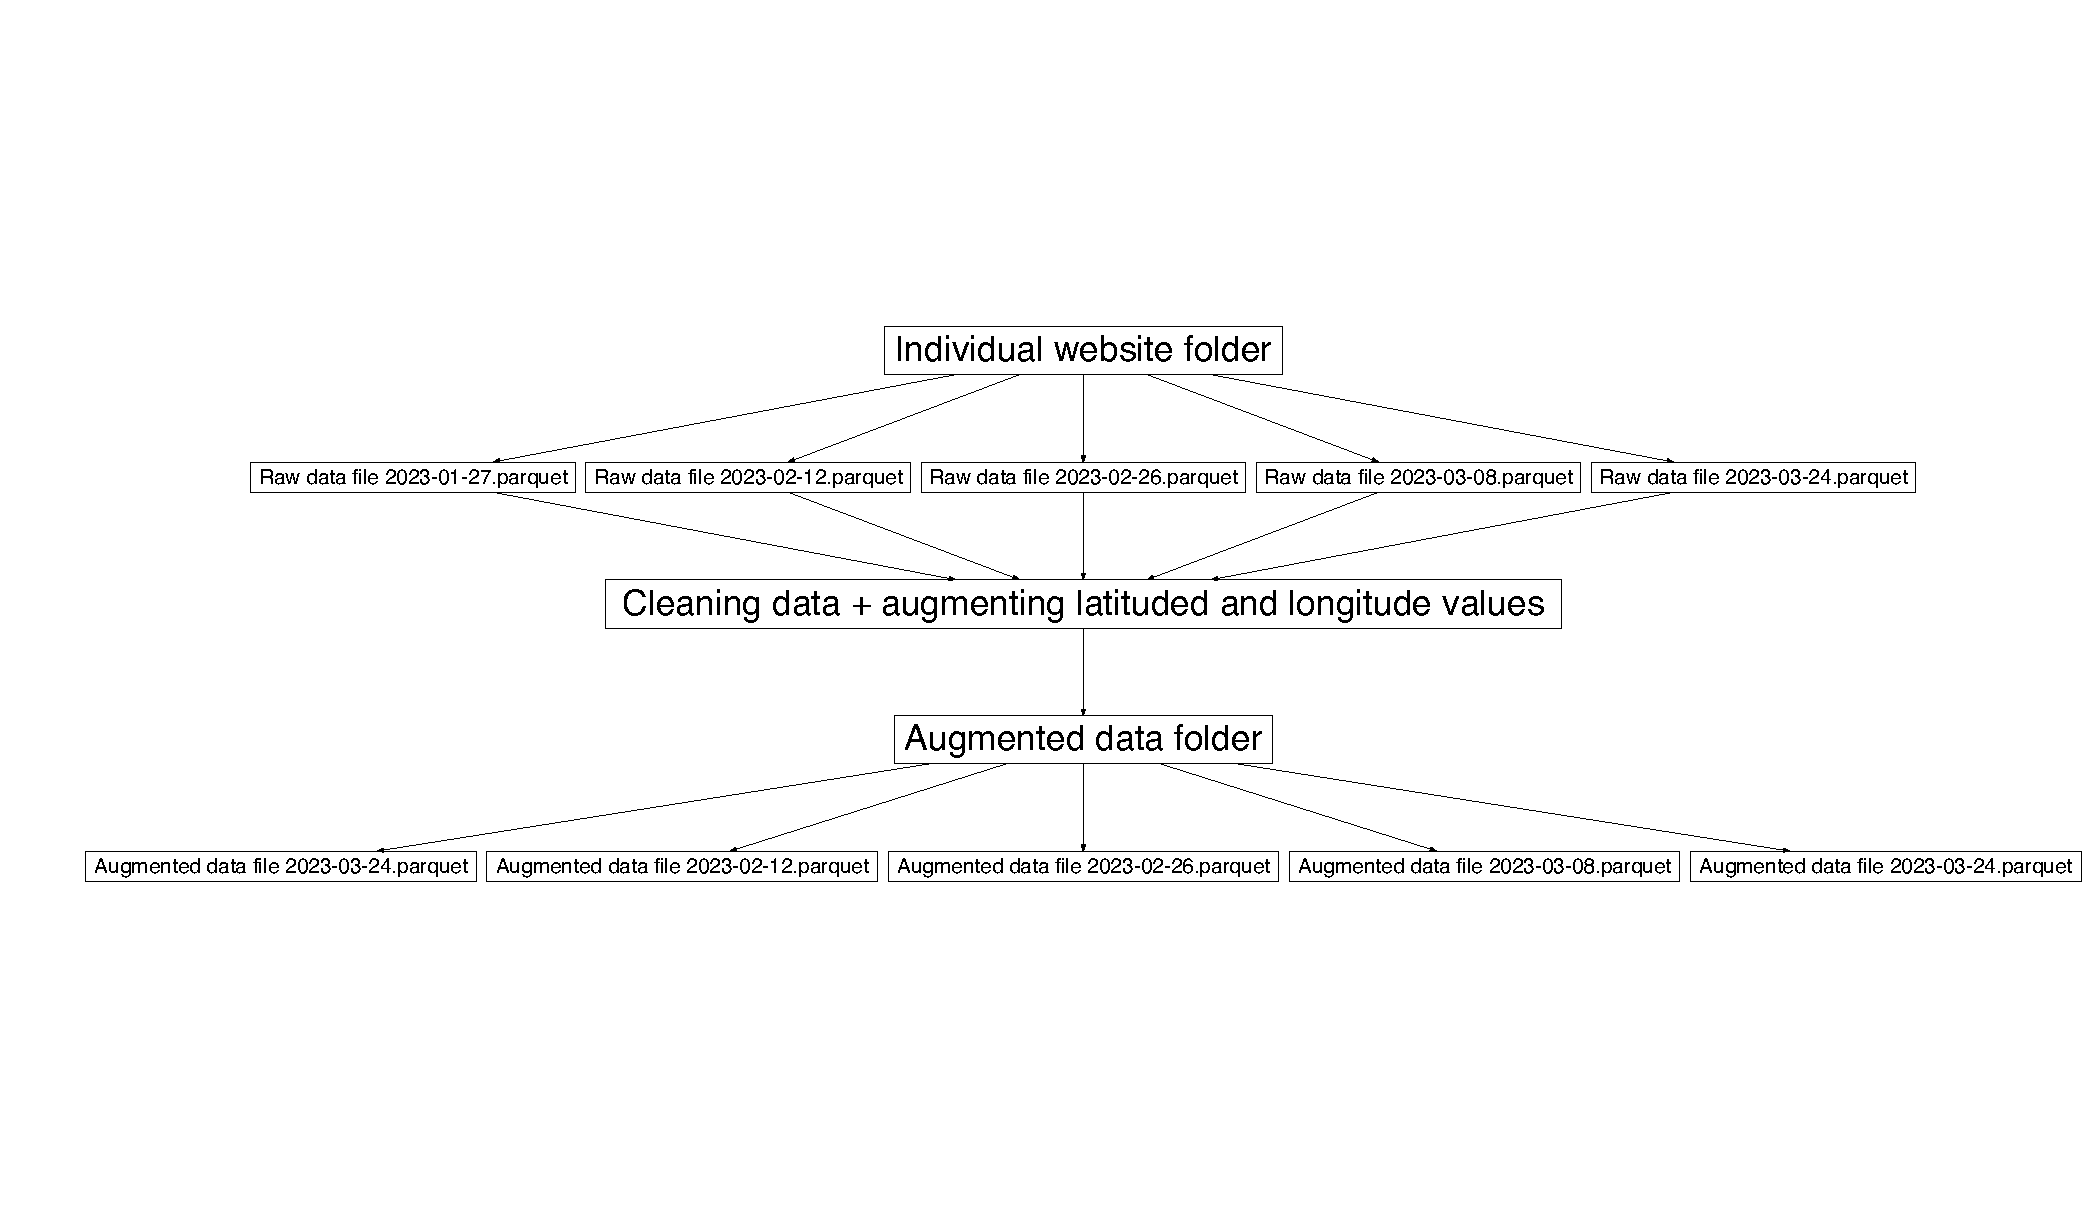
\includegraphics{final_report_files/figure-latex/unnamed-chunk-3-1.pdf}
\caption{Data Storage Flow Chart}
\end{figure}

\hypertarget{data-cleaning}{%
\subsection{Data Cleaning}\label{data-cleaning}}

Figure 3 shows the steps of how the final data was obtained. After the
initial pre-cleaning and data augmentation steps, I combined all parquet
files that live in the augmented data folder. Each website folder has
such a data folder with around 5-6 parquet files. In total there are
around 30 different parquet files with the pre-cleaned data and
augmented latitude and longitude values. I then read in all 30 parquet
files and stacked them on top of each other by row binding them. In the
process I standardized the column names, created new variable that
indicated whether the data comes from a rental website or property price
website, and standardized the property type levels. Afterwards, I
removed missing values and added the neighborhoods to the data frame. In
addition to that I also calculated the distances from properties to the
public places and bus and train stations, and calculated the number of
restaurants and bars and public service places that fall within a 500
meter radius around a property. I also added the number of crimes that
happened in 2021 in each neighborhood to the data set.

\begin{figure}
\centering
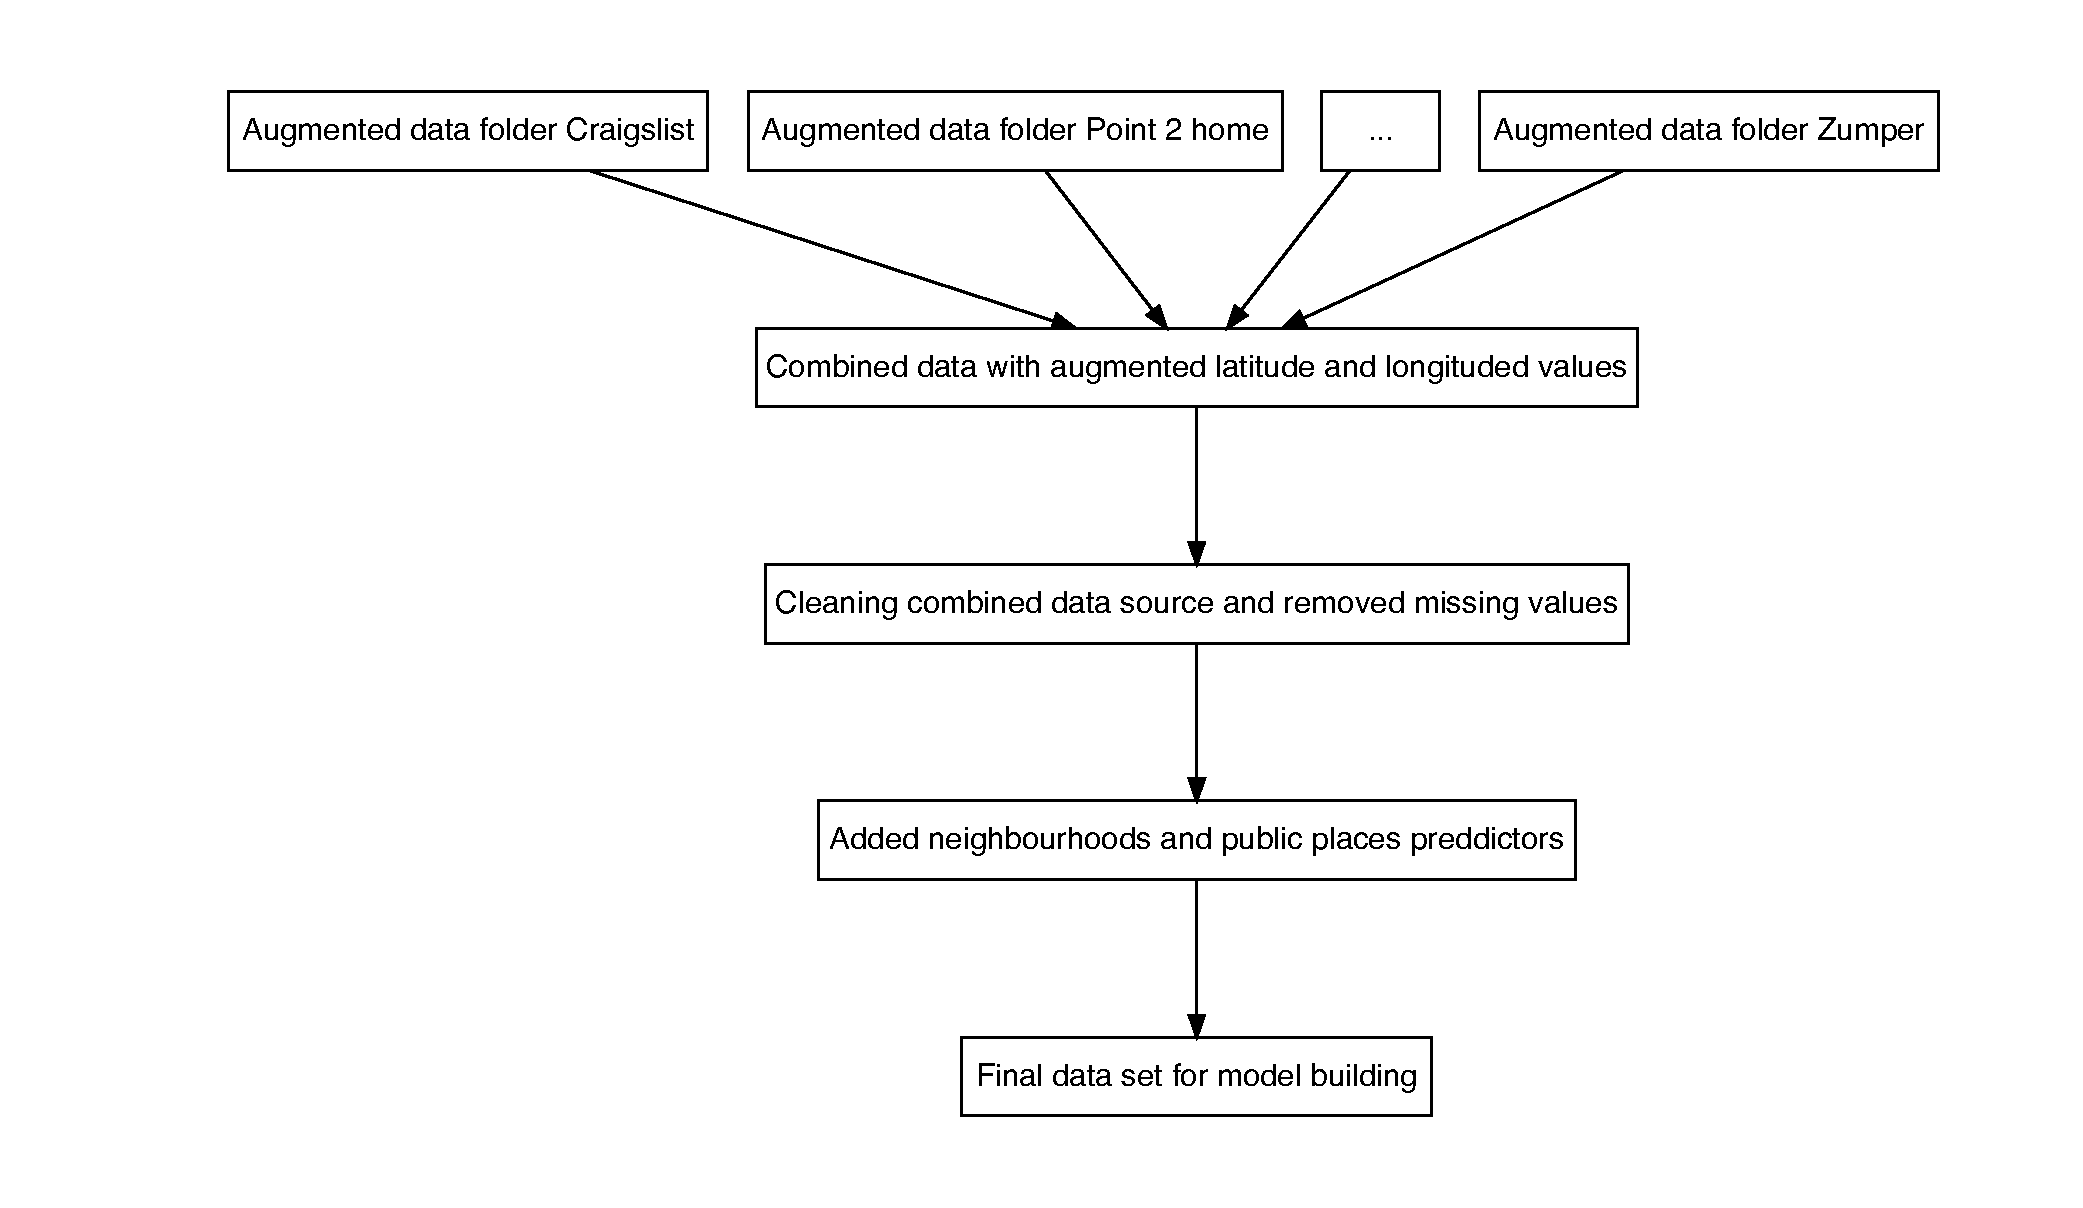
\includegraphics{final_report_files/figure-latex/unnamed-chunk-4-1.pdf}
\caption{Data Cleaning Process Flow Chart}
\end{figure}

\hypertarget{final-data-set}{%
\section{Final Data Set}\label{final-data-set}}

After applying all the filtering steps in the flow chart above I ended
up with around 4000 observations for home prices and 3000 observations
for rental prices.

The predictor variables and their mode are in Table 3. When the property
type is apartment, the lot size will be zero. A more detailed summary
statistics table of all the predictor and response variables can be
found in Table 12 in the Appendix.

\begin{longtable}[]{@{}
  >{\raggedright\arraybackslash}p{(\columnwidth - 2\tabcolsep) * \real{0.8636}}
  >{\raggedright\arraybackslash}p{(\columnwidth - 2\tabcolsep) * \real{0.1364}}@{}}
\caption{Final Predictor Variables}\tabularnewline
\toprule()
\begin{minipage}[b]{\linewidth}\raggedright
Variables From Web Scraping
\end{minipage} & \begin{minipage}[b]{\linewidth}\raggedright
Mode
\end{minipage} \\
\midrule()
\endfirsthead
\toprule()
\begin{minipage}[b]{\linewidth}\raggedright
Variables From Web Scraping
\end{minipage} & \begin{minipage}[b]{\linewidth}\raggedright
Mode
\end{minipage} \\
\midrule()
\endhead
Price & Continuous \\
\# of Bedrooms & Continuous \\
\# of Bathrooms & Continuous \\
\# of Square Feet & Continuous \\
Lot Size in Square Feet & Continuous \\
Latitude & Continuous \\
Longitude & Continuous \\
Closest School (in meters) & Continuous \\
Closest Park (in meters) & Continuous \\
Closest Bus Stop (in meters) & Continuous \\
Closest Sky Train Station (in meters) & Continuous \\
\# of Restaurants/Coffee Shops within 500 meters & Continuous \\
\# of Commercial Services within 500 meters & Continuous \\
\# of Convenience Stores within 500 meters & Continuous \\
\# of Break and Enter Commercial & \\
within neighborhood & Continuous \\
\# of Break and Enter Residential/Other & \\
within neighborhood & Continuous \\
\# of Mischief within neighborhood & Continuous \\
\# Other Theft within neighborhood & Continuous \\
\# Theft from Vehicle within neighborhood & Continuous \\
\# Theft of Bicycle within neighborhood & Continuous \\
\# Theft of Vehicle within neighborhood & Continuous \\
\# Vehicle Collision or Pedestrian Struck (with Injury) & \\
within neighborhood & Continuous \\
Type of Home & Categorical \\
Neighborhood & Categorical \\
Websites & Categorical \\
\bottomrule()
\end{longtable}

\hypertarget{exploratory-data-analysis}{%
\section{Exploratory Data Analysis}\label{exploratory-data-analysis}}

\hypertarget{vancouver-map-and-property-distribution-by-type-and-coloured-by-price}{%
\subsection{Vancouver Map and Property Distribution by Type and Coloured
by
Price}\label{vancouver-map-and-property-distribution-by-type-and-coloured-by-price}}

Figure 4 shows a scatterplot by property type and colored by price. The
most expensive properties are of type house and are located in West
Vancouver. Most of the properties are either apartments or houses. Most
apartments are located in the Downtown area and houses are more randomly
distributed across the Vancouver neighborhoods.

\begin{figure}

{\centering 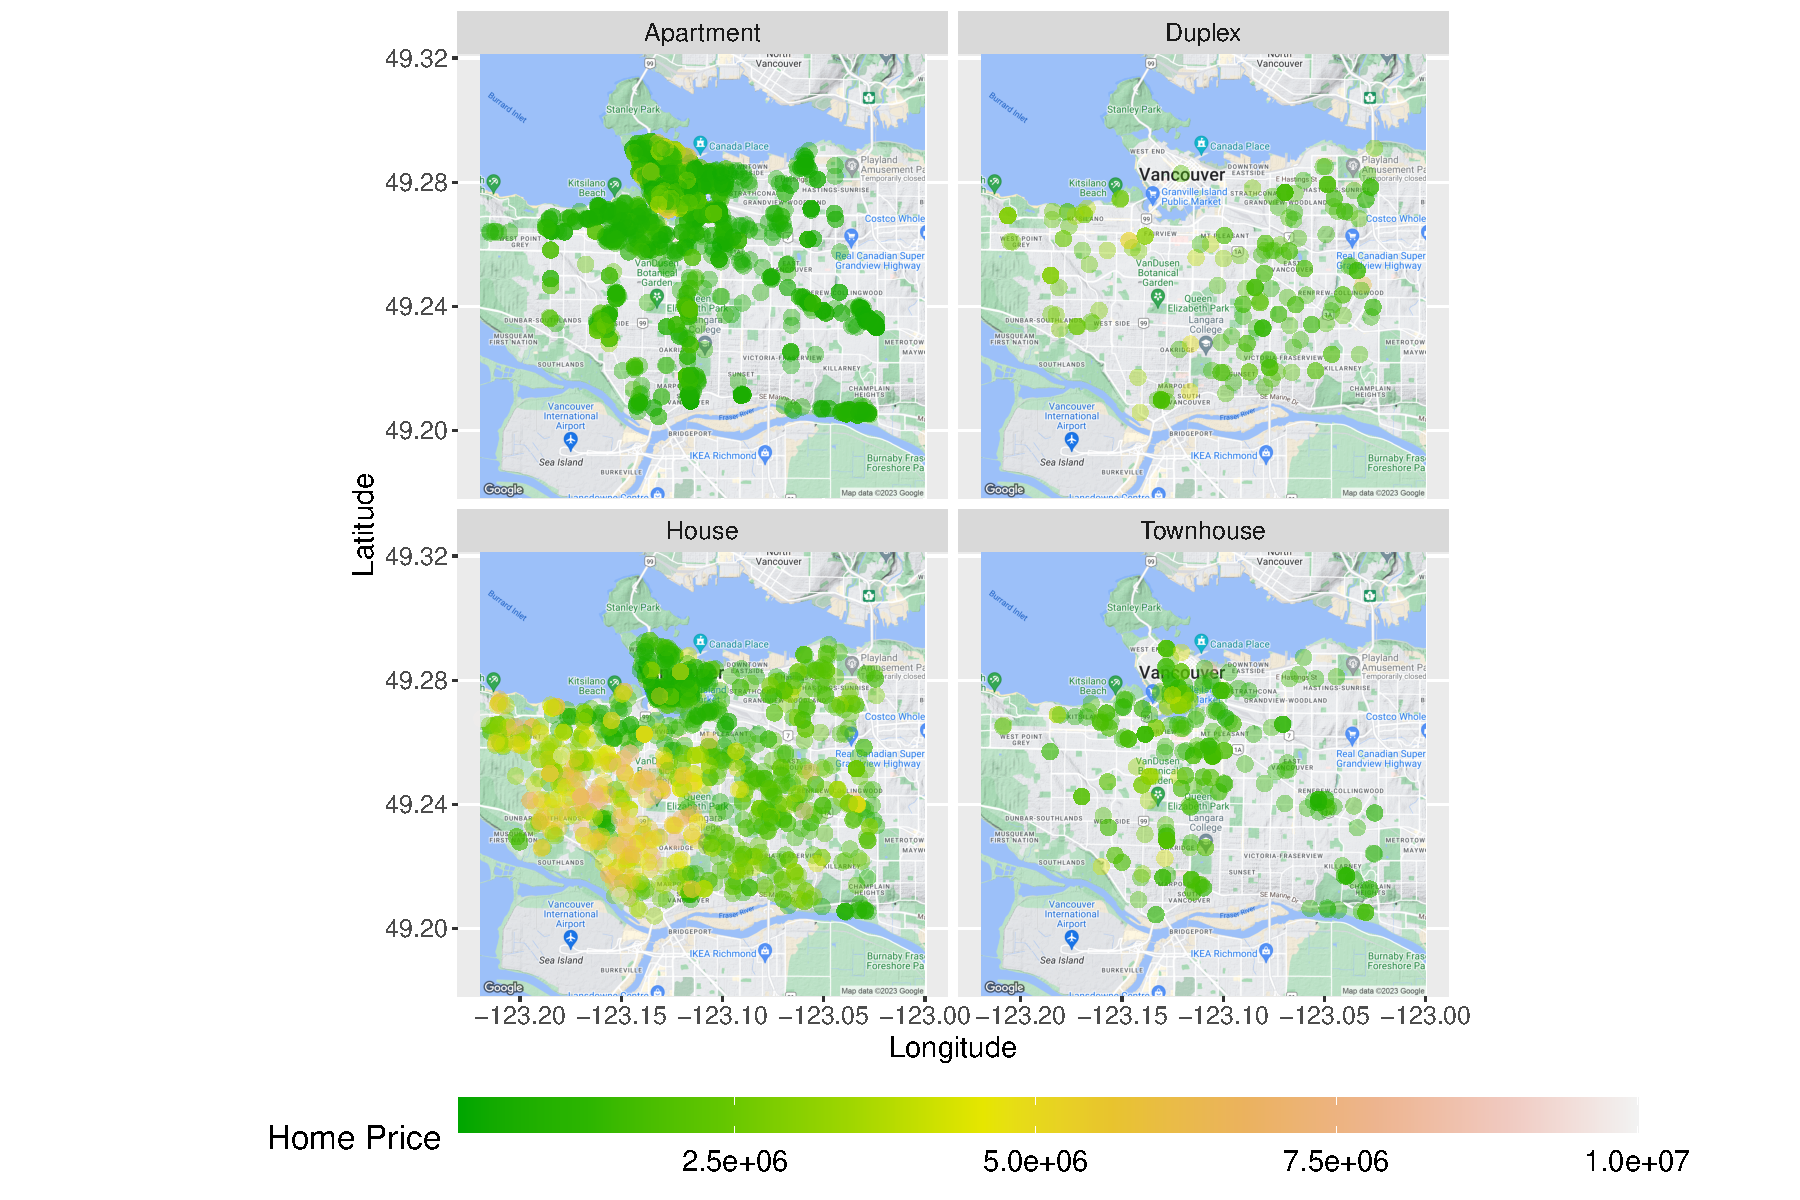
\includegraphics{final_report_files/figure-latex/unnamed-chunk-7-1} 

}

\caption{Density Plot of Price by Proprty Type}\label{fig:unnamed-chunk-7}
\end{figure}

\hypertarget{correlation-matrix}{%
\subsection{Correlation Matrix}\label{correlation-matrix}}

Figure 5 shows a correlation matrix of the response variable, price, and
all other predictors. Longitude is negatively correlated with price. The
higher the price of a property, the less the longitude of a property.
This is in correspondents with Figure 4. The most expensive homes are
located in West Vancouver and therefore, there is a negative correlation
between price and longitude.

It is interesting to see that there is a negative correlation between
price and the number of restaurants and bars and commercial services
near a property. One would think that the more restaurants are near by a
property, the higher the value of a home.

It is also worth noting that there is a positive relationship between
the distance of train stations, bus stations, schools, and parks to a
property. The longer the distance is to these places, the higher the
price of a home.

The negative correlation between crime rates and property prices is
expected. The more crime there is near a property, the lower the price
of the property.

There also is a very high correlation between the number of square feet,
number of baths, number of beds, and the size of the lot of a home to
the price.

\begin{figure}
\centering
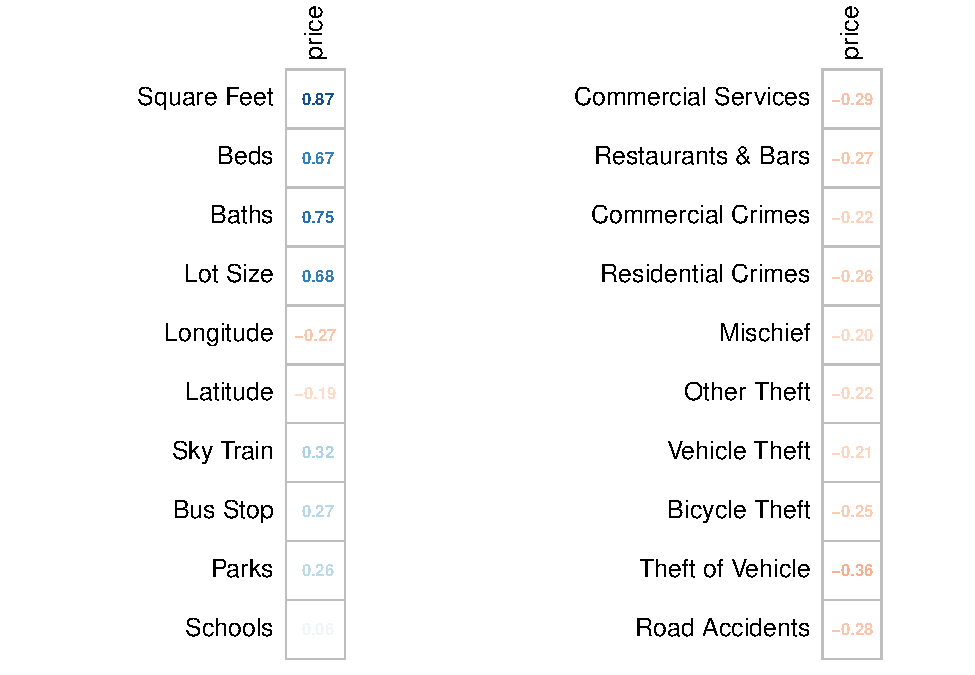
\includegraphics{final_report_files/figure-latex/unnamed-chunk-8-1.pdf}
\caption{Correlation Matrix Between the Response Variable and
Predictors}
\end{figure}

\hypertarget{deep-dive-into-correlations}{%
\subsection{Deep Dive Into
Correlations}\label{deep-dive-into-correlations}}

Figure 6 shows that there are different relationships between the price
of a property and how many commercial services are near a home, by
property type. The higher the number of commercial services near a
house, the less that property is worth. In contrast, there does not seem
to be a relationship for other property types. However, for apartments,
the price of a property increases if there are more than 200 commercial
services near by.

\begin{figure}
\centering
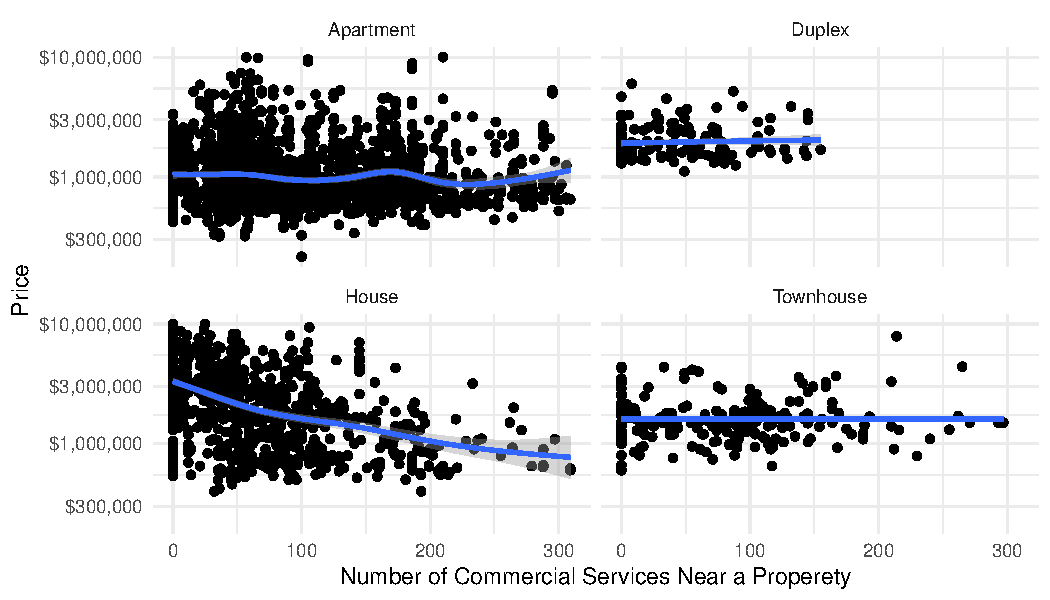
\includegraphics{final_report_files/figure-latex/unnamed-chunk-9-1.pdf}
\caption{Scattreplot of Price and Commercial Services by Property Type}
\end{figure}

Similarly, Figure 7 shows the relationship between the distance in
meters from a property to a train station. There is a strong positive
relationship between the distance of a house and the nearest train
station. For apartments, the relationship varies depending on how far
away the train station is. The plot shows that there is a slight
positive relationship from around 0-800 meters with price, and then a
slight negative relationship from 800 meters to 2000 meters. This
suggests that apartments right next to a sky train station are valued
less. On the other hand, apartments increase in value until around 800
meters, then the price decreases from 800 to 2000 meters.

\begin{figure}
\centering
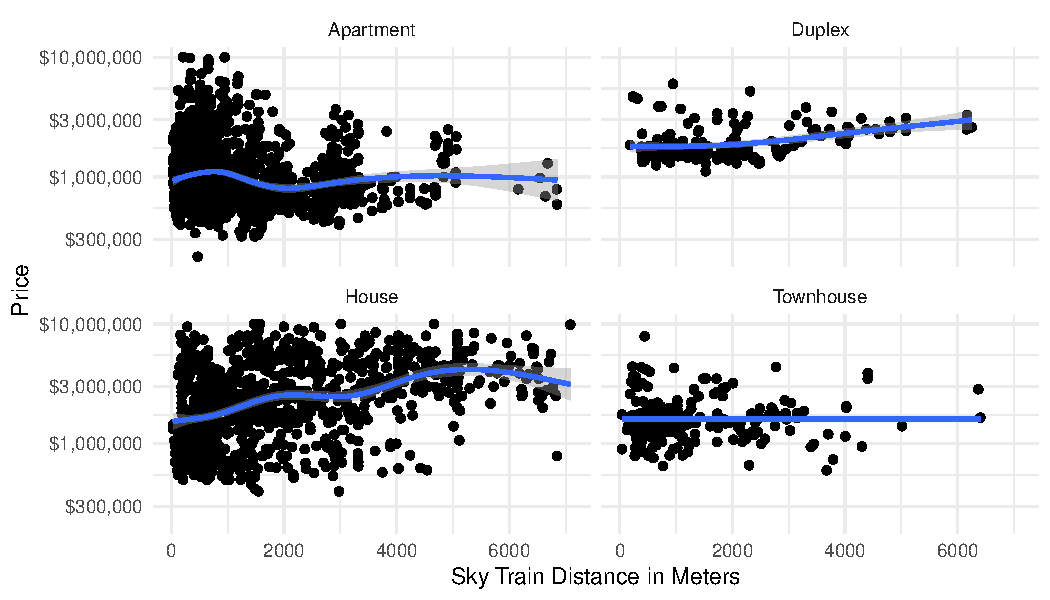
\includegraphics{final_report_files/figure-latex/unnamed-chunk-10-1.pdf}
\caption{Scattreplot of Price and Distance to the Nearest Sky Train
Station By Property Type}
\end{figure}

Figure 8 shows the strongest correlation between the response variable
price and the predictor square feet. The higher the number of square
feet, the higher valued a property is.

\begin{figure}
\centering
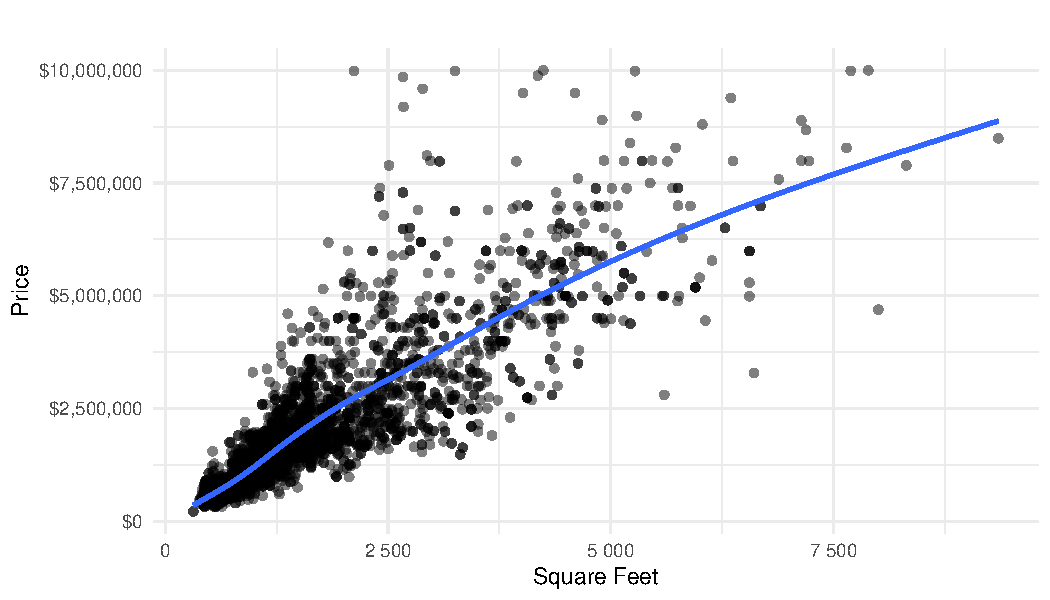
\includegraphics{final_report_files/figure-latex/unnamed-chunk-11-1.pdf}
\caption{Scattreplot of Price and Square Feet}
\end{figure}

\newpage

\hypertarget{data-biases-from-scraped-websites}{%
\subsection{Data Biases From Scraped
Websites}\label{data-biases-from-scraped-websites}}

Figure 9 shows a box plot of the price of a property by website and
property type. It is interesting to see that duplexes are more expensive
on Remax compared to Zolo and Rew. Also, home prices on Point 2 Home are
less expensive compared to Zolo and Rew. This could lead to some biases
in the final model and also suggests that it is important to include the
website as a categorical predictor to mitigate this bias. To reduce this
bias, we should include the website as a categorical predictor in the
model.

\begin{figure}
\centering
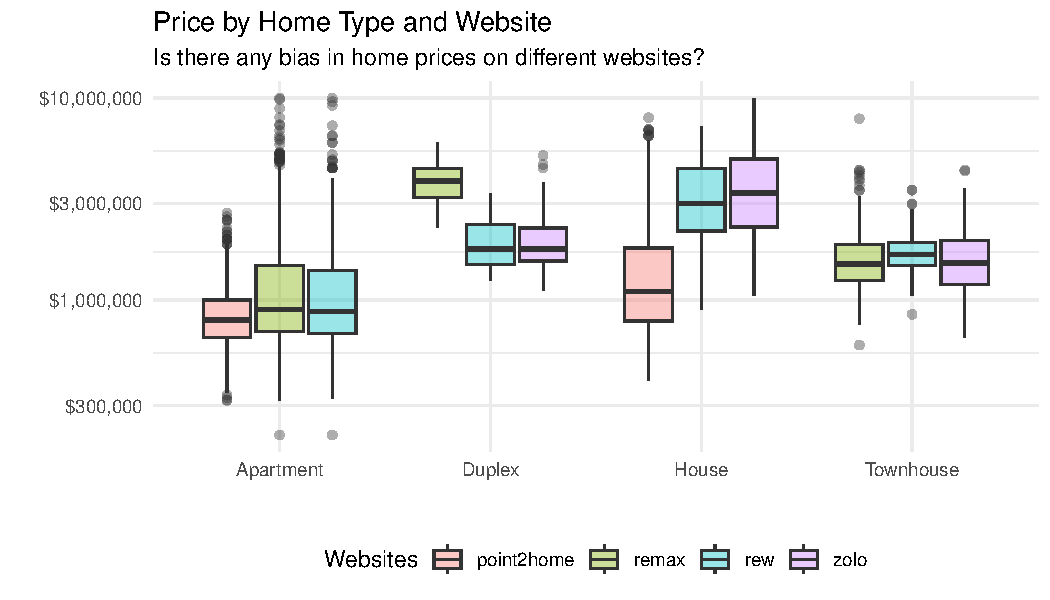
\includegraphics{final_report_files/figure-latex/unnamed-chunk-12-1.pdf}
\caption{Boxplot of Prices by Homes and Websites}
\end{figure}

\hypertarget{interaction-effects}{%
\subsection{Interaction Effects}\label{interaction-effects}}

When looking at interactions, I decided to run a MARS model with the
\texttt{earth} package for all numerical variables in the data set. For
this, I set up a grid with two hyperparameters. One for the number of
interactions that the model should consider and the second one for how
many predictor variables there should be in the model. For this, I used
the caret package and 10-fold cross-validation to choose the best
hyperparameters. Figure 10 and Table 4 show the results of the
cross-validation process. Table 5 shows the most important interaction
effects according to the MARS model.

\begin{figure}
\centering
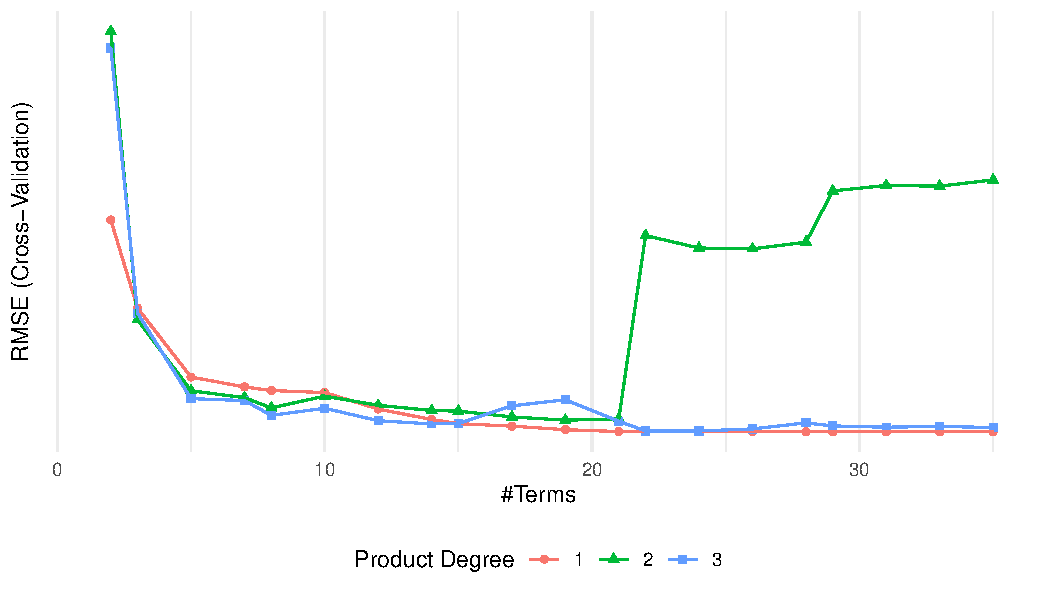
\includegraphics{final_report_files/figure-latex/unnamed-chunk-13-1.pdf}
\caption{Cross-Validation Results for MARS Model}
\end{figure}

Because I would like to see if there are any interaction effects in the
data, I decided to choose the model with degree three and 31 parameters
in the model.

\begin{longtable}[]{@{}rrll@{}}
\caption{MARS Cross-Validation Results}\tabularnewline
\toprule()
degree & nprune & MAE & RMSE \\
\midrule()
\endfirsthead
\toprule()
degree & nprune & MAE & RMSE \\
\midrule()
\endhead
1 & 26 & \$396,922 & \$656,184 \\
1 & 28 & \$396,922 & \$656,184 \\
2 & 19 & \$369,664 & \$664,109 \\
2 & 21 & \$370,197 & \$665,026 \\
3 & 31 & \$352,925 & \$659,327 \\
3 & 35 & \$353,024 & \$659,101 \\
\bottomrule()
\end{longtable}

\begin{longtable}[]{@{}
  >{\raggedright\arraybackslash}p{(\columnwidth - 2\tabcolsep) * \real{0.8205}}
  >{\raggedleft\arraybackslash}p{(\columnwidth - 2\tabcolsep) * \real{0.1795}}@{}}
\caption{Interaction Effects Chosen by the MARS
Algorithm}\tabularnewline
\toprule()
\begin{minipage}[b]{\linewidth}\raggedright
preds
\end{minipage} & \begin{minipage}[b]{\linewidth}\raggedleft
price
\end{minipage} \\
\midrule()
\endfirsthead
\toprule()
\begin{minipage}[b]{\linewidth}\raggedright
preds
\end{minipage} & \begin{minipage}[b]{\linewidth}\raggedleft
price
\end{minipage} \\
\midrule()
\endhead
h(3392-square\_feet)*h(lng--123.13) & 9016.4038262 \\
h(square\_feet-2398)*h(lng--123.078) & 41081.8173697 \\
h(square\_feet-2398)*h(-123.078-lng) & 10629.9884373 \\
h(square\_feet-2398)\emph{h(4-baths)}h(-123.078-lng) & -5743.2219997 \\
h(square\_feet-1057)\emph{h(2000-lot\_size)}h(lat-49.259) &
16.0431959 \\
h(lot\_size-2000)*h(598.367-sky\_train) & 2.6005060 \\
h(lot\_size-2000)\emph{h(598.367-sky\_train)}h(27-commercial\_services)
& -0.0444601 \\
h(lot\_size-2000)\emph{h(lat-49.2284)}h(598.367-sky\_train) &
-49.5962353 \\
\bottomrule()
\end{longtable}

In Figure 11, the most interesting interactions are displayed. The
interactions are modeled with a GAM model and the tensor product between
the two predictors, displayed in each plot, was used.

In the upper left plot, square feet are displayed on the x-axis and
longitude on the y-axis. It is interesting to see that for high and low
longitude values and high square feet, properties are the most
expensive. However, for longitude values in the middle range, properties
are not as expensive as for extreme values for longitude. This might be
because of a bad neighborhood for these longitude values.

The upper right plot shows lot size on the y-axis and how far the
nearest sky train station is away from a property on the x-axis. It is
noticeable that prices are highest for large lots that are far away from
sky train stations. Properties that are very close to sky train stations
and have large lots are not valued as much. It is interesting to see a
bump in the plot for lot sizes in the middle ranges and properties that
are near a sky train station but not right next to one. Probably of the
noise, people do not value living next to a sky train station but there
seems to be a sweet spot where people value a close distance to a nearby
sky train station.

The middle left corner shows latitude on the x-axis and lot size on the
y-axis. The plot looks similar to the square feet and longitude plot.
For extreme values of latitude and a large lot size, properties are
expensive. For the middle range of values for latitude, lot size does
not matter as much.

The middle right plot shows the number of commercial services near a
property on the y-axis and the sky train distance on the x-axis.
Property prices do not vary much for properties very close to a sky
train station for any number of commercial services and are valued
highly when being far away from a sky train station and having no
commercial services around. These properties are most likely very
expensive single-family homes in rural areas.

The lower left plot shows the interaction between square feet and
longitude, accounting for all predictor variables in the model.
Adjusting for these variables, the interaction effect looks very
different. I believe, that the main reason for this behavior is that lot
size, square feet, and neighborhood explain a lot of the variation in
housing prices and therefore, the type of a home effect is less strong.

Similarly for lot size and the nearest sky train station. There is
generally a trend where the farther away the sky train station is, the
more expensive a home and also the greater the lot size the more
expensive a property is.

\begin{figure}
\centering
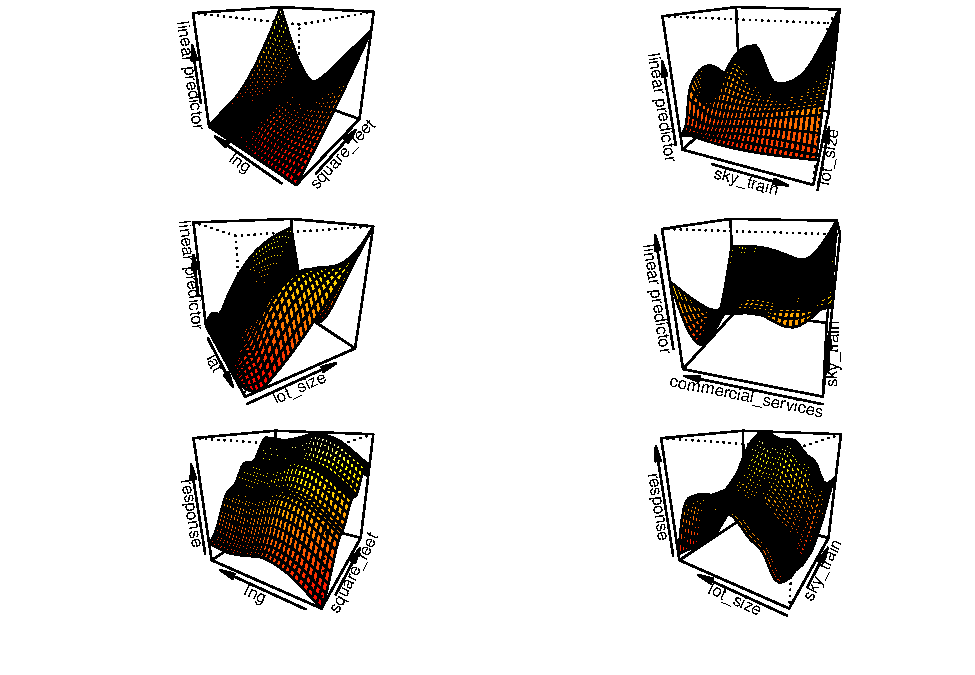
\includegraphics{final_report_files/figure-latex/unnamed-chunk-16-1.pdf}
\caption{Interaction Effects In Hosuing Data}
\end{figure}

\hypertarget{partial-effects-of-gam-model}{%
\subsection{Partial Effects of GAM
Model}\label{partial-effects-of-gam-model}}

\begin{figure}
\centering
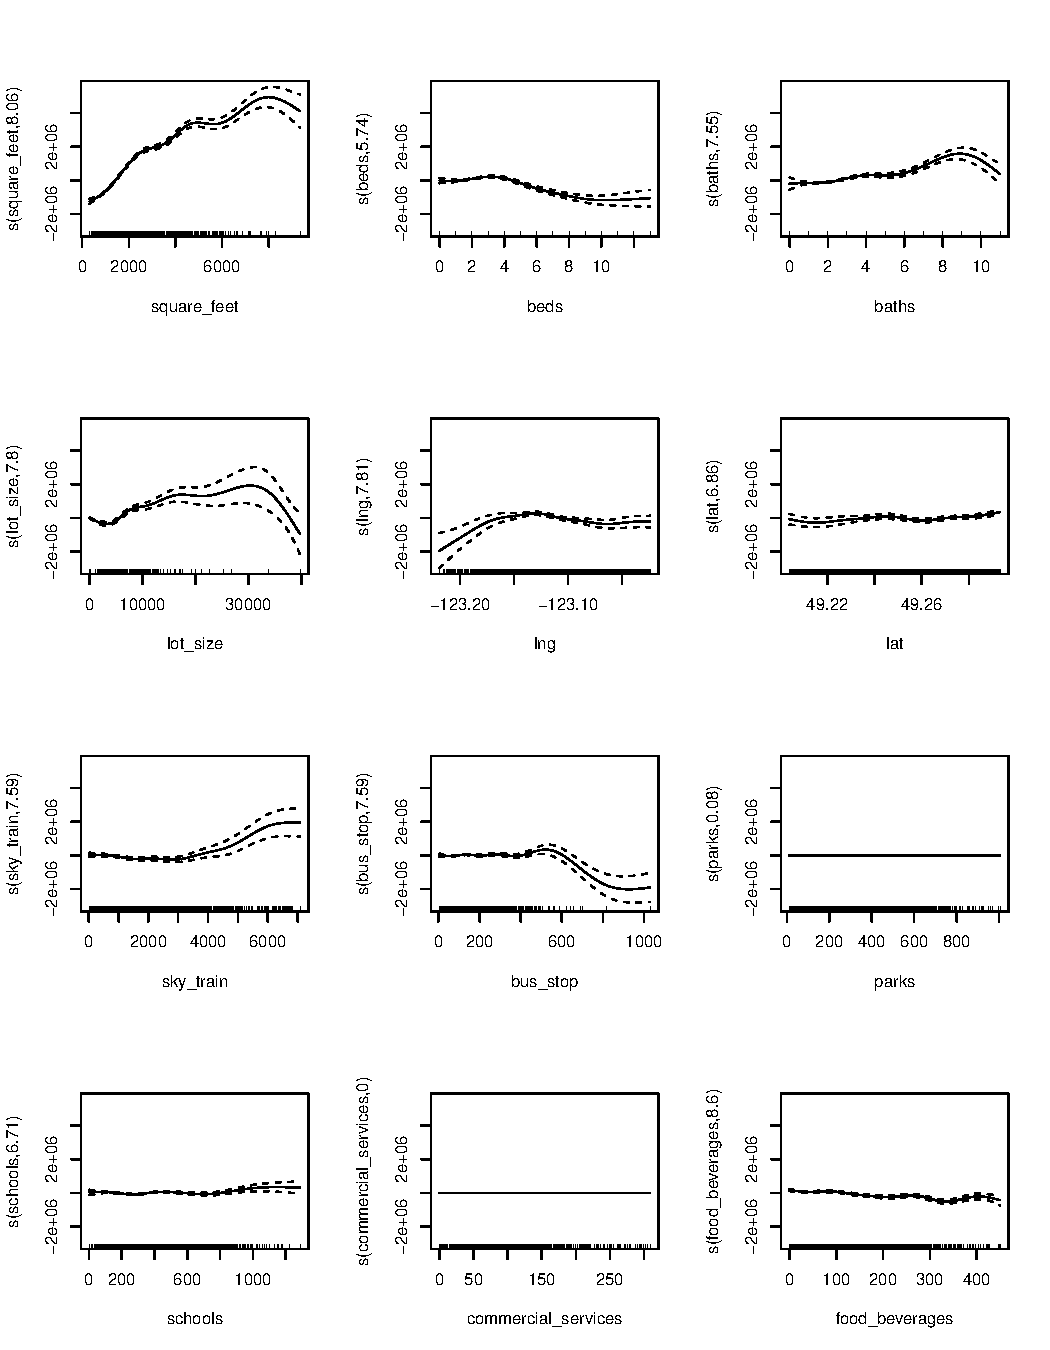
\includegraphics{final_report_files/figure-latex/unnamed-chunk-17-1.pdf}
\caption{Partial Effects From GAM Model Where Smoothed Out Predictors
Were Omitted}
\end{figure}

Figure 12 shows the most interesting partial effects where all
predictors that were smoothed out by the penalty term were omitted. The
fitted GAM model used all predictors shown in Table 3.

We can see that for square feet, the partial effects correspond to
Figure 8 where with increasing square feet, the price of a property
increases.

For the sky train stations, there is a slight decrease in the value of a
property the greater the distance between a property and the nearest sky
train station. The price increases when a sky train station is more than
3000 meters away from a property. When someone is familiar with
Vancouver and the train stations, then one knows that sky train stations
are far away from West Vancouver where the most expensive properties are
located according to Figure 4. So seeing the value of a home increase
after 3000 meters is expected. Interestingly, the value of properties
decreases dramatically when a property is farther away than 600 meters
from the nearest bus stop.

It is also interesting to see that the higher the longitude value, the
higher the price of a home. This is contrary to the correlation plot,
Figure 4, and the density map, Figure 5, where we see that expensive
homes are located in the west of Vancouver. Figure 13 shows a GAM model
on the left-hand side with only longitude as predictor and on the right
hand-side, neighborhood, the type of the property, square feet, and lot
size were added as predictor variables. Adjusting for these variables,
the longitude effect is not as high anymore. This explains the longitude
graph in Figure 12 where all predictors were included in the GAM model.

\begin{figure}
\centering
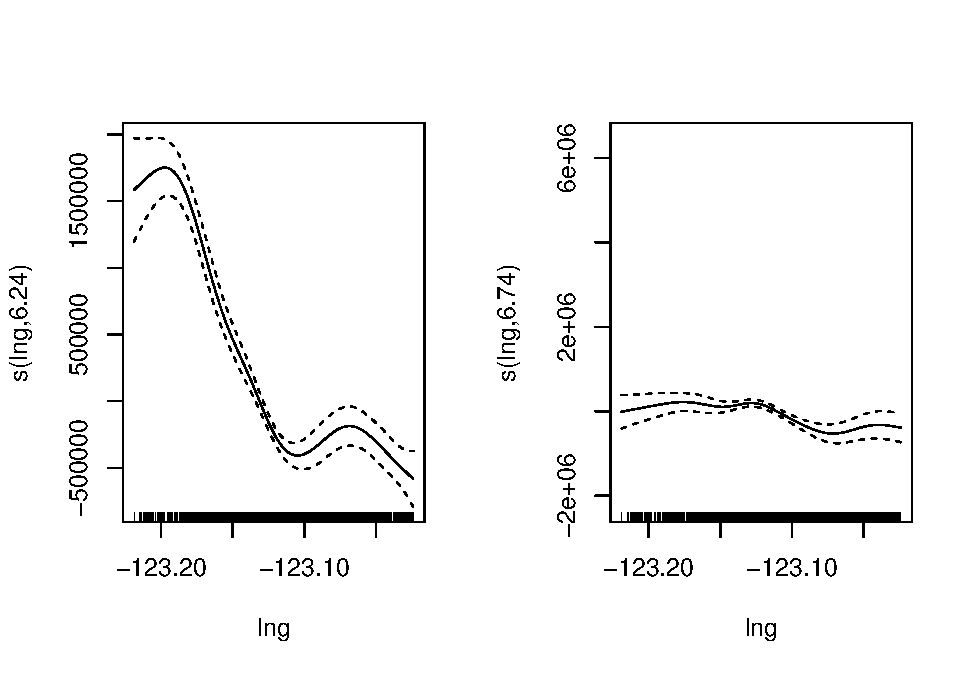
\includegraphics{final_report_files/figure-latex/unnamed-chunk-18-1.pdf}
\caption{The left-hand side plot displays a GAM model with price as the
response variable and longitude as the only predictor variable. As seen
in Figure 4 and Figure 5, the lower the longitude, the higher the price.
The right-hand side plot adjusts for the property type, neeighborhood,
square feet, and lot size. We can see that adjusting for these
variables, the effect of longitude flattens out.}
\end{figure}

\newpage

\hypertarget{statistical-analysis}{%
\section{Statistical Analysis}\label{statistical-analysis}}

\hypertarget{data-preprocessing}{%
\subsection{Data Preprocessing}\label{data-preprocessing}}

I divided the data into a training and a testing data set. 80\% of the
data is for training and 20\% is for testing. In addition to that, 80\%
of the training data was split into 10 equal data sets to perform
10-fold cross-validation to tune the hyperparameters. All data
pre-processing steps are done separately for folds and testing data to
avoid data leakage. The pre-processing steps involved one hot encoding
for dummy variables and then normalizing all predictor variables.

\hypertarget{random-forest}{%
\subsection{Random Forest}\label{random-forest}}

The first model that I built is a random forest model where I tuned
three hyperparameters. The libraries I used were \texttt{tidymodels} and
\texttt{ranger}. I used Latin Hypercube samples and a grid of 30
observations for the three tuning parameters. The results of the
hypereparameter tuning are shown in Figure 14.

There are no improvements in the number of trees or randomly selected
predictors. However, the smaller the node size, the lower the mean
absolute error and the higher the r-squared value. Therefore I set the
range for the minimal node size between one and eight and used a Latin
Hypercube grid to tune the hyperparameters for a second time. The
results of the hyperparameter tuning for the second run are shown in
Figure 15.

\begin{figure}
\centering
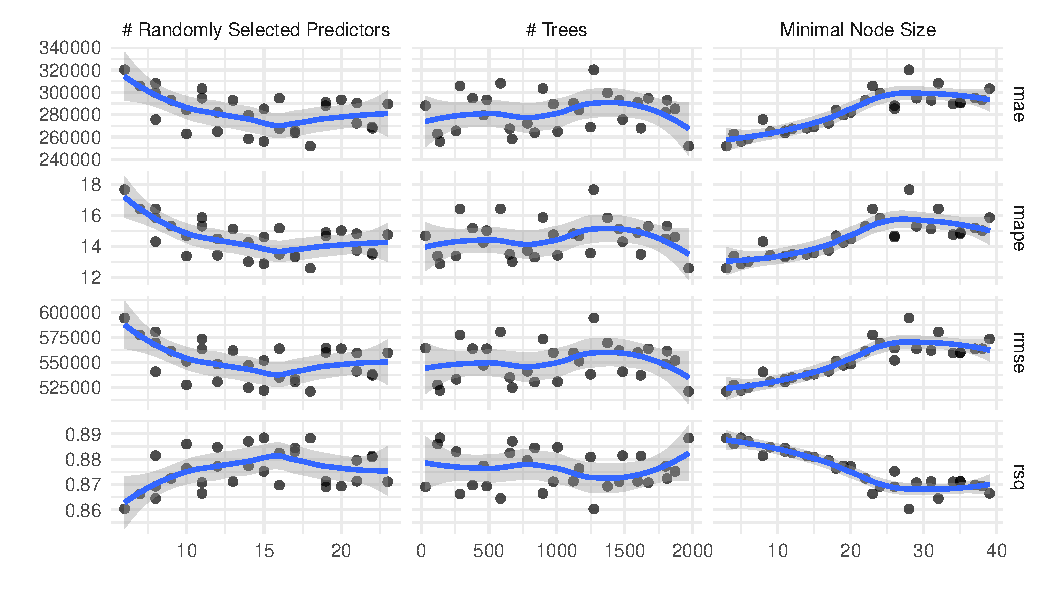
\includegraphics{final_report_files/figure-latex/unnamed-chunk-22-1.pdf}
\caption{Tuning Parametrs Random Forest After Initial Grid}
\end{figure}

Based on the plot, the lowest mean absolute error occurs when there are
between 20 and 25 predictors selected and the minimal node size is
between one and three.

\begin{figure}
\centering
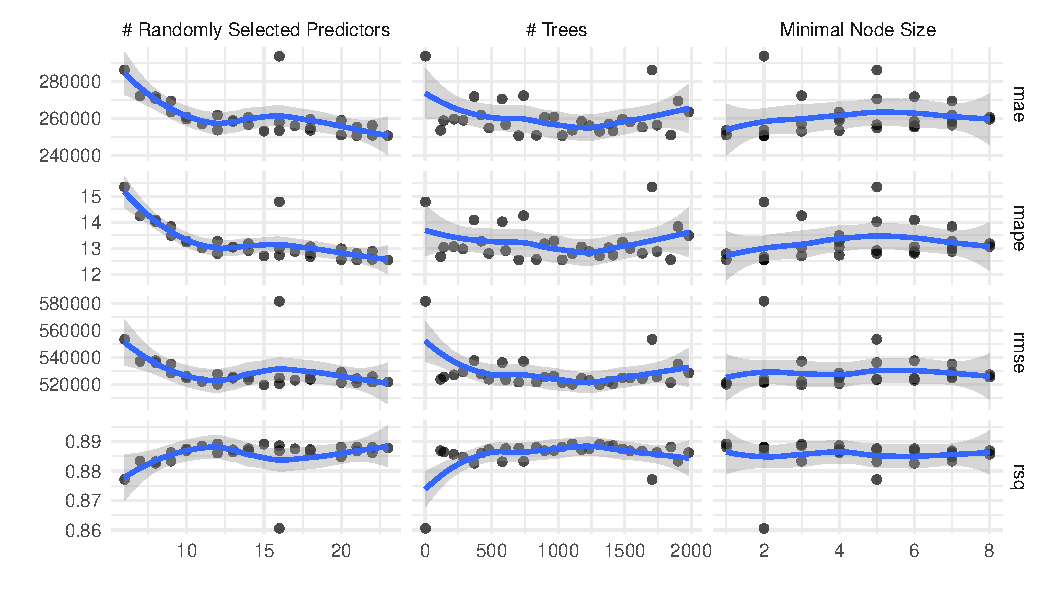
\includegraphics{final_report_files/figure-latex/unnamed-chunk-24-1.pdf}
\caption{Tuning Paramatres Random Forest Scond Run After Grid
Optimization}
\end{figure}

Table 6 shows the results of the best model. The best model has 21
predictors, 1031 trees, and a node size of two. After determining the
best hyperparameters through 10-fold cross-validation by choosing the
model with the lowest mean absolute error, the final model is trained on
the full 80\% of training data and evaluated on the 20\% of testing
data.

\begin{longtable}[]{@{}
  >{\raggedleft\arraybackslash}p{(\columnwidth - 12\tabcolsep) * \real{0.2532}}
  >{\raggedleft\arraybackslash}p{(\columnwidth - 12\tabcolsep) * \real{0.0759}}
  >{\raggedleft\arraybackslash}p{(\columnwidth - 12\tabcolsep) * \real{0.2278}}
  >{\raggedright\arraybackslash}p{(\columnwidth - 12\tabcolsep) * \real{0.1139}}
  >{\raggedright\arraybackslash}p{(\columnwidth - 12\tabcolsep) * \real{0.0886}}
  >{\raggedright\arraybackslash}p{(\columnwidth - 12\tabcolsep) * \real{0.1139}}
  >{\raggedright\arraybackslash}p{(\columnwidth - 12\tabcolsep) * \real{0.1266}}@{}}
\caption{Coss-Validation Results for Random Forest}\tabularnewline
\toprule()
\begin{minipage}[b]{\linewidth}\raggedleft
Predictors Selected
\end{minipage} & \begin{minipage}[b]{\linewidth}\raggedleft
Trees
\end{minipage} & \begin{minipage}[b]{\linewidth}\raggedleft
Minimum Node Size
\end{minipage} & \begin{minipage}[b]{\linewidth}\raggedright
MAE
\end{minipage} & \begin{minipage}[b]{\linewidth}\raggedright
MAPE
\end{minipage} & \begin{minipage}[b]{\linewidth}\raggedright
RMSE
\end{minipage} & \begin{minipage}[b]{\linewidth}\raggedright
R-SQUARED
\end{minipage} \\
\midrule()
\endfirsthead
\toprule()
\begin{minipage}[b]{\linewidth}\raggedleft
Predictors Selected
\end{minipage} & \begin{minipage}[b]{\linewidth}\raggedleft
Trees
\end{minipage} & \begin{minipage}[b]{\linewidth}\raggedleft
Minimum Node Size
\end{minipage} & \begin{minipage}[b]{\linewidth}\raggedright
MAE
\end{minipage} & \begin{minipage}[b]{\linewidth}\raggedright
MAPE
\end{minipage} & \begin{minipage}[b]{\linewidth}\raggedright
RMSE
\end{minipage} & \begin{minipage}[b]{\linewidth}\raggedright
R-SQUARED
\end{minipage} \\
\midrule()
\endhead
21 & 1031 & 2 & \$250,598 & 12.55\% & \$521,292 & 88.82\% \\
\bottomrule()
\end{longtable}

Table 7 shows the results of the testing data. The mean absolute error
is \$221,627 dollars, the mean absolute percentage error is 11.83\%, and
the r-squared value is 91.27\%. This means that all the predictors
explain around 91\% of the variation in prices in the test set.

\begin{longtable}[]{@{}lllll@{}}
\caption{Random Forest Results For Testing data}\tabularnewline
\toprule()
Model & MAE & MAPE & RMSE & R-SQUARED \\
\midrule()
\endfirsthead
\toprule()
Model & MAE & MAPE & RMSE & R-SQUARED \\
\midrule()
\endhead
Random Forest & \$221,627 & 11.83\% & \$441,444 & 91.27\% \\
\bottomrule()
\end{longtable}

\newpage

\hypertarget{variable-importance-random-forest}{%
\subsubsection{Variable Importance Random
Forest}\label{variable-importance-random-forest}}

Figure 16 shows the 15 most important variables determined by the random
forest model. Square feet is the most important predictor when
determining the price of a property followed by lot size, baths, beds,
longitude, the distance to the nearest sky train station, the distance
to the nearest park, latitude, and if a website came from a Zolo listing
or not. It is interesting that the type of a home is not very important
relative to other predictors. The lot size is probably explaining the
variation in price better than the property type.

\begin{figure}
\centering
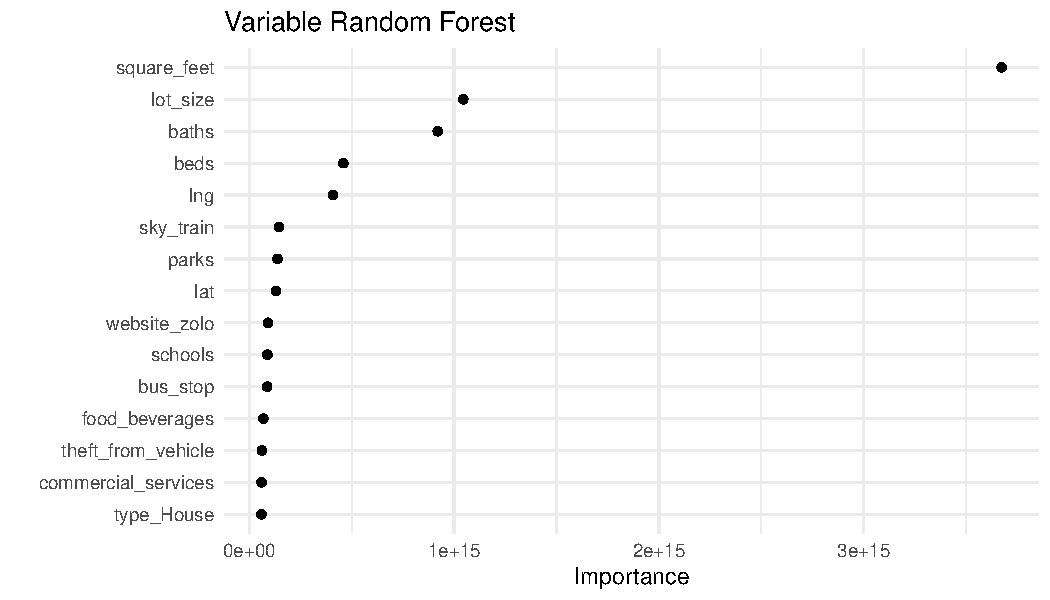
\includegraphics{final_report_files/figure-latex/unnamed-chunk-30-1.pdf}
\caption{Variable Importance Random Forest}
\end{figure}

\hypertarget{gradient-boosted-decision-tree}{%
\subsection{Gradient Boosted Decision
Tree}\label{gradient-boosted-decision-tree}}

The second model that I evaluated was a gradient-boosted decision tree.
The hyperparameters I tuned for this model were the tree depth, the
minimum node size, loss reduction, learning rate, sample size, and the
number of predictors chosen. I again used a Latin Hypercube to sample 20
observations. I set the range of the number of predictors chosen from
six to the number of predictors in the data set and the learning rate
from 0.003 to 0.27.

In Figure 17 we see the values of the hyperparameters associated with
the different metrics. From the plot, I concluded that 1-15 predictors
give the best mean absolute error combined when 60\% to 90\% of the
samples are selected. Moreover, a node size between 1 and 10 gives the
lowest mean absolute error.

In the next round of tuning, I added these changes and sampled 20
observations from a Grid Latin Hypercube, and started the 10-fold
cross-validation again to determine the best hyperparameters. The
results are shown in Figure 18.

\begin{figure}
\centering
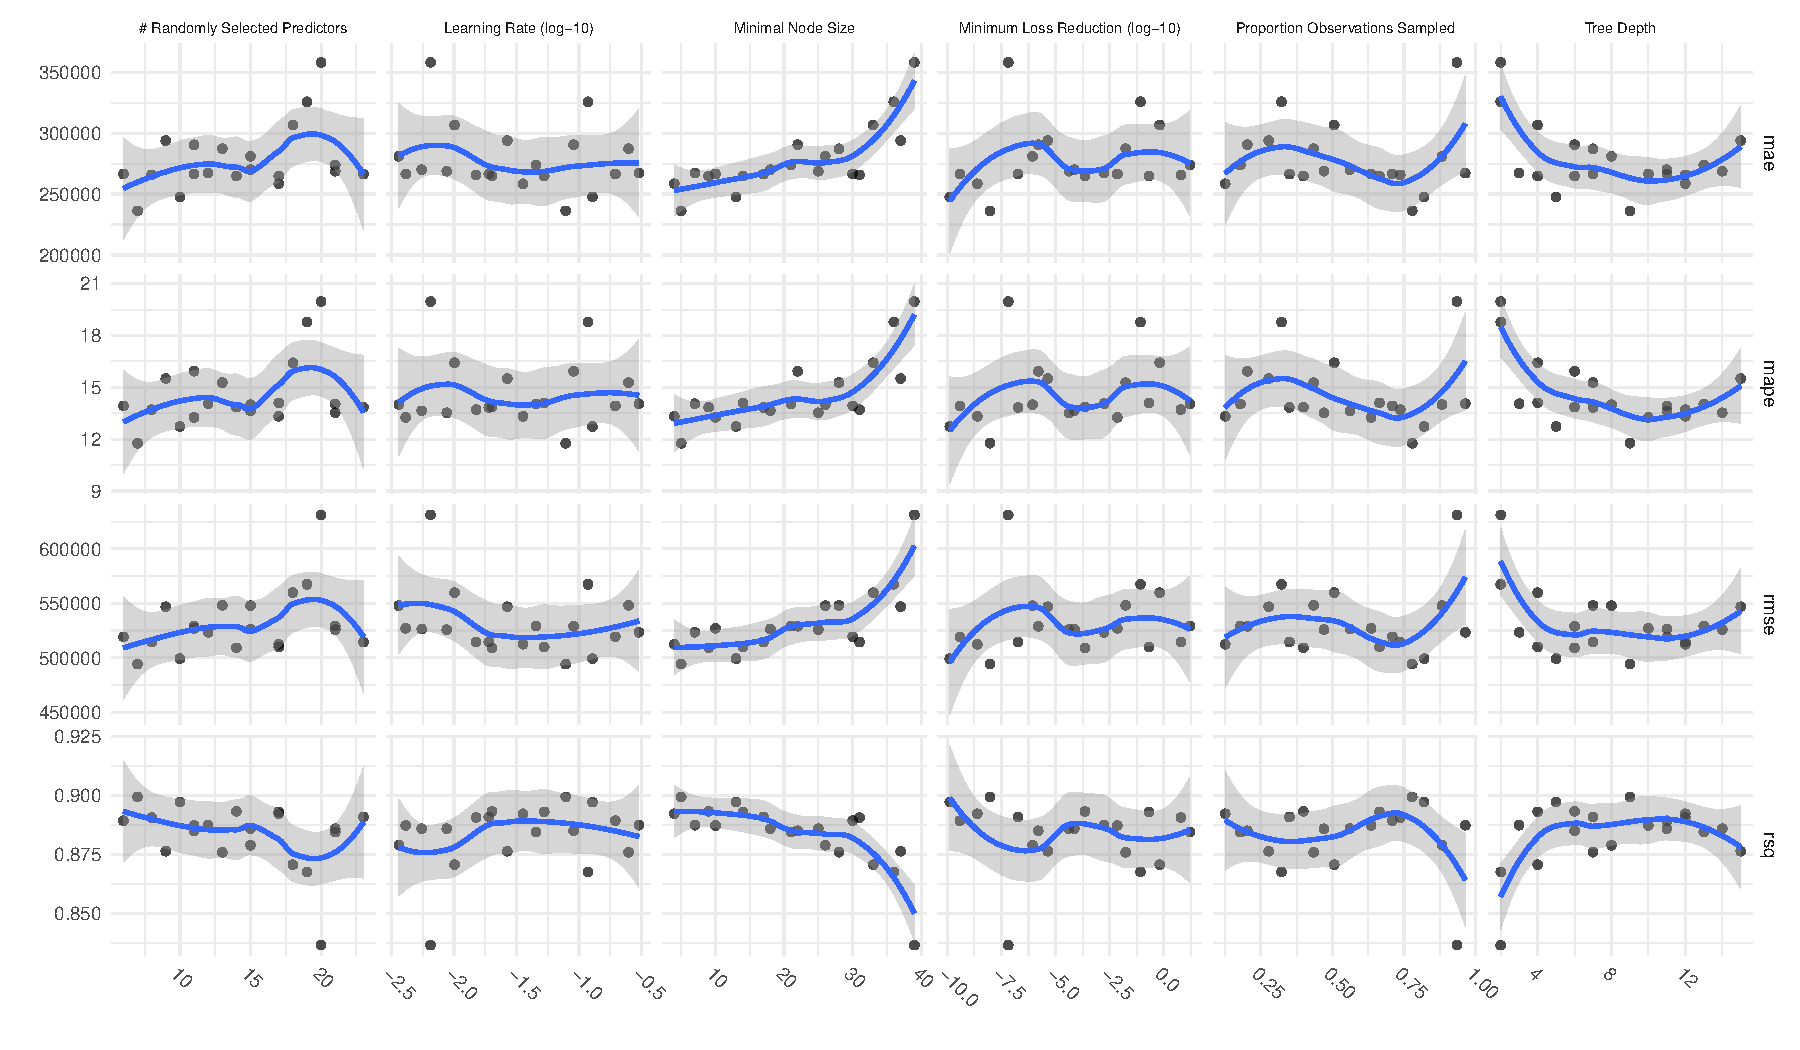
\includegraphics{final_report_files/figure-latex/unnamed-chunk-32-1.pdf}
\caption{XG Boost Hyperparamters After First Run}
\end{figure}

\begin{figure}
\centering
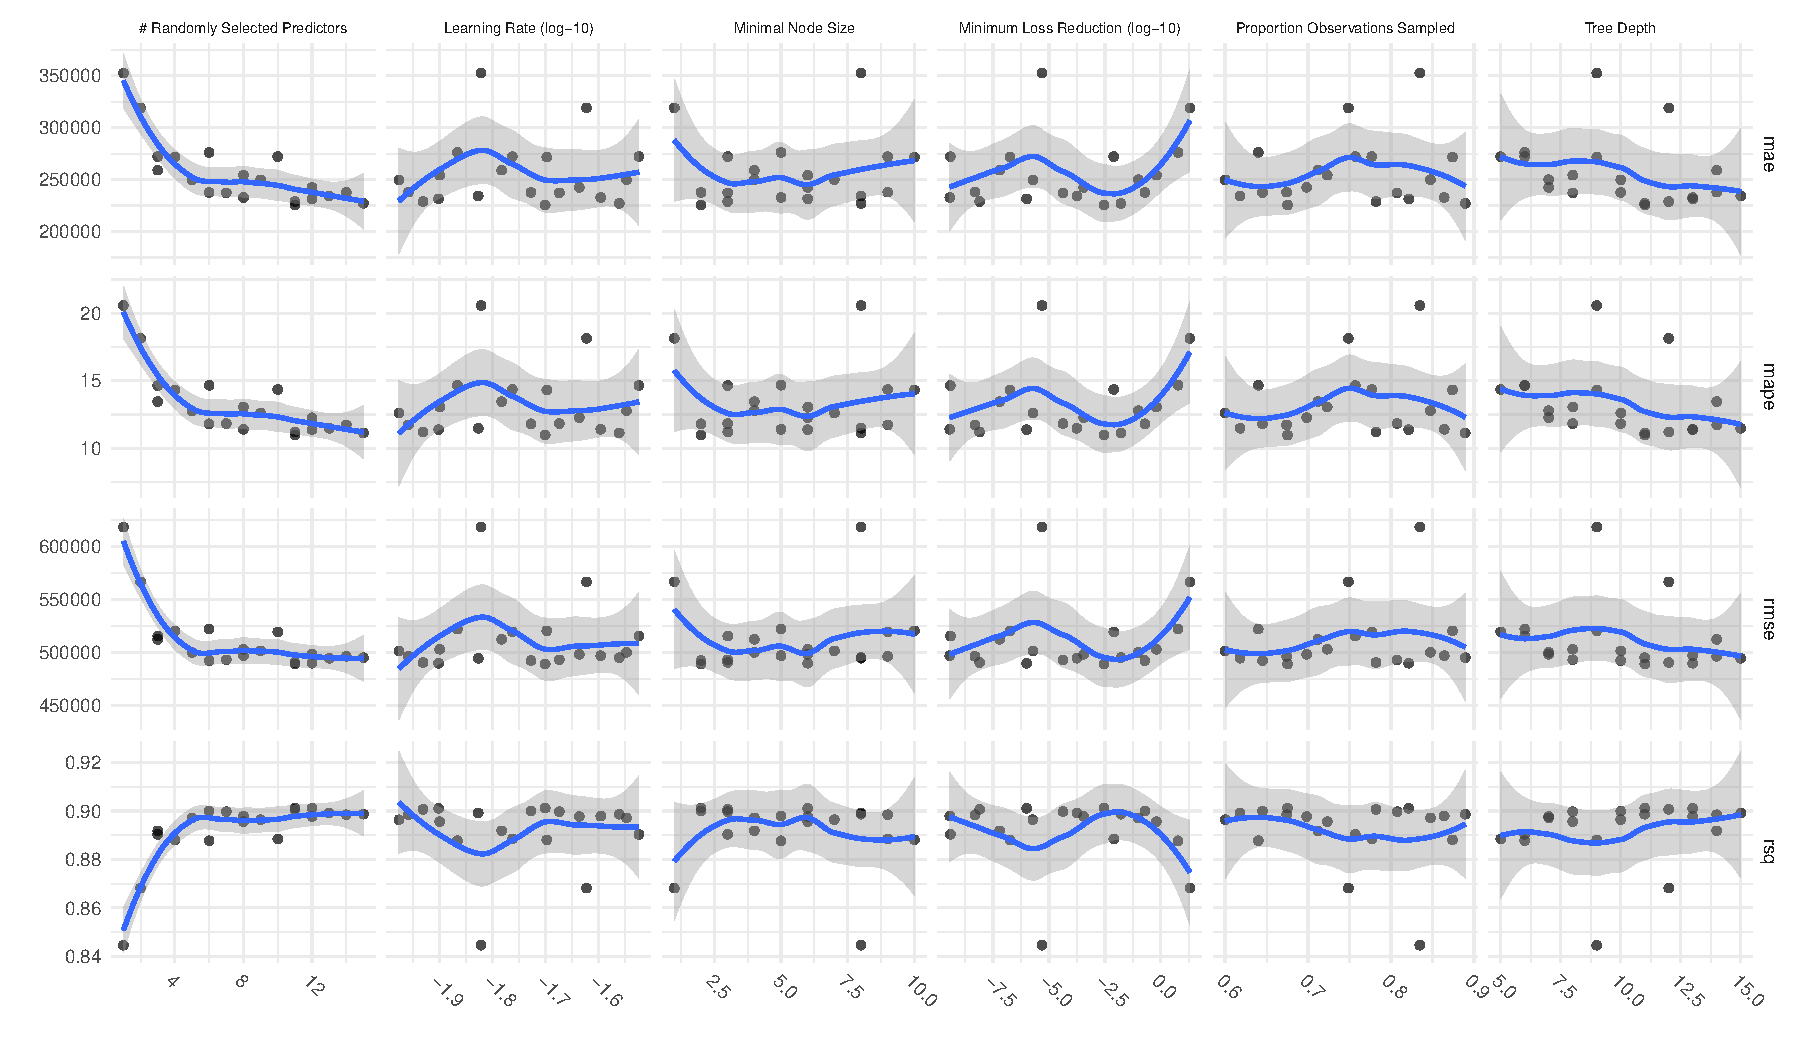
\includegraphics{final_report_files/figure-latex/unnamed-chunk-34-1.pdf}
\caption{XG Boost Hyperparamters After Seccond Run}
\end{figure}

Table 8 shows the results of the best model from cross-validation. The
final model is trained on the full 80\% of training data and evaluated
on the 20\% of testing data.

\begin{longtable}[]{@{}
  >{\raggedleft\arraybackslash}p{(\columnwidth - 18\tabcolsep) * \real{0.1368}}
  >{\raggedleft\arraybackslash}p{(\columnwidth - 18\tabcolsep) * \real{0.1197}}
  >{\raggedleft\arraybackslash}p{(\columnwidth - 18\tabcolsep) * \real{0.0940}}
  >{\raggedleft\arraybackslash}p{(\columnwidth - 18\tabcolsep) * \real{0.1197}}
  >{\raggedleft\arraybackslash}p{(\columnwidth - 18\tabcolsep) * \real{0.1282}}
  >{\raggedleft\arraybackslash}p{(\columnwidth - 18\tabcolsep) * \real{0.1026}}
  >{\raggedright\arraybackslash}p{(\columnwidth - 18\tabcolsep) * \real{0.0769}}
  >{\raggedright\arraybackslash}p{(\columnwidth - 18\tabcolsep) * \real{0.0598}}
  >{\raggedright\arraybackslash}p{(\columnwidth - 18\tabcolsep) * \real{0.0769}}
  >{\raggedright\arraybackslash}p{(\columnwidth - 18\tabcolsep) * \real{0.0855}}@{}}
\caption{XG Boost Results For Cross Validation Data}\tabularnewline
\toprule()
\begin{minipage}[b]{\linewidth}\raggedleft
\# of Predictors
\end{minipage} & \begin{minipage}[b]{\linewidth}\raggedleft
Min Node Size
\end{minipage} & \begin{minipage}[b]{\linewidth}\raggedleft
Tree Depth
\end{minipage} & \begin{minipage}[b]{\linewidth}\raggedleft
Learning Rate
\end{minipage} & \begin{minipage}[b]{\linewidth}\raggedleft
Loss Reduction
\end{minipage} & \begin{minipage}[b]{\linewidth}\raggedleft
Sample Size
\end{minipage} & \begin{minipage}[b]{\linewidth}\raggedright
MAE
\end{minipage} & \begin{minipage}[b]{\linewidth}\raggedright
MAPE
\end{minipage} & \begin{minipage}[b]{\linewidth}\raggedright
RMSE
\end{minipage} & \begin{minipage}[b]{\linewidth}\raggedright
R-SQUARED
\end{minipage} \\
\midrule()
\endfirsthead
\toprule()
\begin{minipage}[b]{\linewidth}\raggedleft
\# of Predictors
\end{minipage} & \begin{minipage}[b]{\linewidth}\raggedleft
Min Node Size
\end{minipage} & \begin{minipage}[b]{\linewidth}\raggedleft
Tree Depth
\end{minipage} & \begin{minipage}[b]{\linewidth}\raggedleft
Learning Rate
\end{minipage} & \begin{minipage}[b]{\linewidth}\raggedleft
Loss Reduction
\end{minipage} & \begin{minipage}[b]{\linewidth}\raggedleft
Sample Size
\end{minipage} & \begin{minipage}[b]{\linewidth}\raggedright
MAE
\end{minipage} & \begin{minipage}[b]{\linewidth}\raggedright
MAPE
\end{minipage} & \begin{minipage}[b]{\linewidth}\raggedright
RMSE
\end{minipage} & \begin{minipage}[b]{\linewidth}\raggedright
R-SQUARED
\end{minipage} \\
\midrule()
\endhead
11 & 2 & 11 & 0.0199 & 0.0029 & 0.6753 & \$225,509 & 10.97\% & \$489,203
& 90.12\% \\
\bottomrule()
\end{longtable}

Table 9 shows the results of the testing data. The mean absolute error
is \$202,887 dollars, the mean absolute percentage error is 10.32\%, and
the r-squared value is 91.69\%. This means that all the predictors
explain around 92\% of the variation in prices in the test set.

\begin{longtable}[]{@{}lllll@{}}
\caption{XG Boost Results For Testing Data}\tabularnewline
\toprule()
Model & MAE & MAPE & RMSE & R-SQUARED \\
\midrule()
\endfirsthead
\toprule()
Model & MAE & MAPE & RMSE & R-SQUARED \\
\midrule()
\endhead
XG Boost & \$202,887 & 10.32\% & \$431,133 & 91.69\% \\
\bottomrule()
\end{longtable}

\hypertarget{variable-importance-xg-boost}{%
\subsubsection{Variable Importance XG
Boost}\label{variable-importance-xg-boost}}

\begin{figure}
\centering
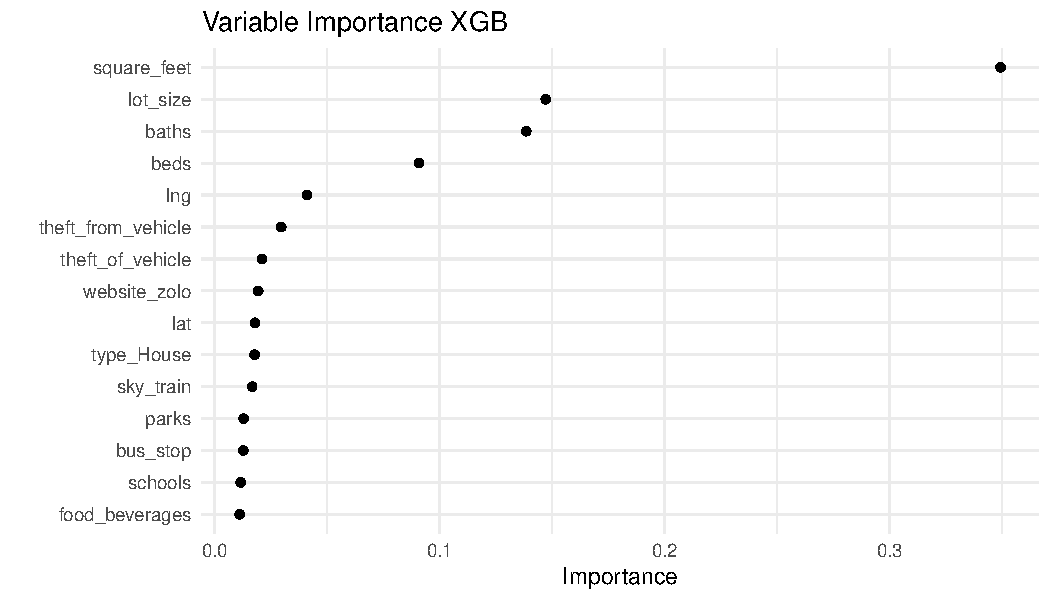
\includegraphics{final_report_files/figure-latex/unnamed-chunk-38-1.pdf}
\caption{Variable Importance of Gradient Boosted Decision Tree}
\end{figure}

Variable importance between the random forest and the XG boost model
look very similar. However, it is interesting to note that some crime
variables are higher ranked for the XG boost model compared to the
random forest.

Both models agree on the the ranks one to five. The random forest goes
with the sky train variable for rank six and parks for rank seven
followed by latitude for rank eight. The XG boost model ranks theft from
vehicle and theft of vehicle as number six and seven respectively
followed by if a website is listed on Zolo or not. The predictors
latitude, sky train, and parks are ranked nine, ten, and eleven
respectively.

\hypertarget{model-comparison}{%
\section{Model Comparison}\label{model-comparison}}

From Figure 20 we can conclude that both models did well when predicting
price. The correlation between the actual price and the predictions is
around 96\% for both models. The gradient-boosted decision tree does
slightly better than the random forest model.

\begin{figure}
\centering
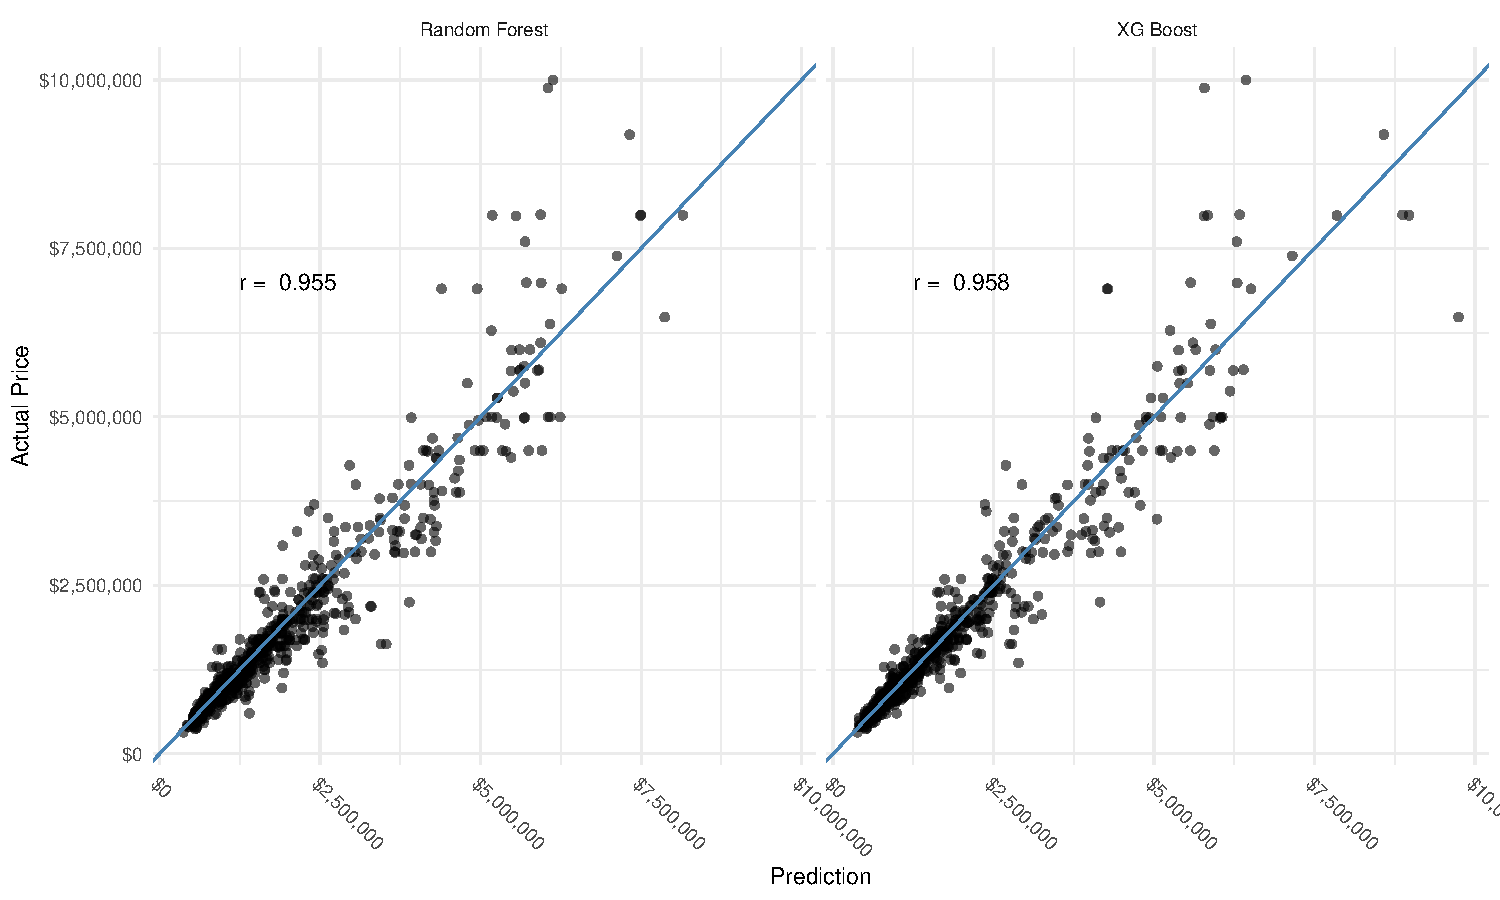
\includegraphics{final_report_files/figure-latex/unnamed-chunk-39-1.pdf}
\caption{Actual Property Prices Versus Predictions}
\end{figure}

Table 10 summarizes the results for the cross-validation score and also
the score for predicting the test set.

Both models predicted listing prices very well. Especially for property
listing prices below \$2,500,000 dollars, the correlation between
predicted and actual listing prices is very high. For listing prices
higher than \$5,000,000 dollars, the random forest model underestimated
most of the listing prices. This is because most of the dots are above
the blue line for the random forest model.

We see a similar behavior for the boosted tree model. For listing prices
higher than \$5,000,000 dollars, the boosted tree model also
underestimated most of the listing prices. However, it appears that is
does not underestimated the prices as much as the random forest model.
This is because visually it seems that more of the dots are below the
blue line for a price point greater than \$5,000,000 dollars when
comparing it to the random forest graph. Also, for the gradient-boosted
tree model, it looks like the correlation between predicted and actual
listing prices is higher for properties below \$2,500,000 dollars. The
dots seem to be closer to the blue line without as much variation as in
the random forest plot.

Overall, both models are very similar and the gradient-boosted decision
tree does slightly better than the random forest. Also, both models
roughly rank the predictors in similar order. Based on the mean absolute
error for the cross-validation data and test set data, I would choose
the gradient boosted decision tree over the random forest. The only
disadvantage is additional compute time due to more hyperparameters.

\begin{longtable}[]{@{}
  >{\raggedright\arraybackslash}p{(\columnwidth - 10\tabcolsep) * \real{0.2121}}
  >{\raggedright\arraybackslash}p{(\columnwidth - 10\tabcolsep) * \real{0.1364}}
  >{\raggedright\arraybackslash}p{(\columnwidth - 10\tabcolsep) * \real{0.1061}}
  >{\raggedright\arraybackslash}p{(\columnwidth - 10\tabcolsep) * \real{0.1364}}
  >{\raggedright\arraybackslash}p{(\columnwidth - 10\tabcolsep) * \real{0.1515}}
  >{\raggedright\arraybackslash}p{(\columnwidth - 10\tabcolsep) * \real{0.2576}}@{}}
\caption{Model Results Of Cross-Validation and Testing Data
Sets}\tabularnewline
\toprule()
\begin{minipage}[b]{\linewidth}\raggedright
Model
\end{minipage} & \begin{minipage}[b]{\linewidth}\raggedright
MAE
\end{minipage} & \begin{minipage}[b]{\linewidth}\raggedright
MAPE
\end{minipage} & \begin{minipage}[b]{\linewidth}\raggedright
RMSE
\end{minipage} & \begin{minipage}[b]{\linewidth}\raggedright
R-SQUARED
\end{minipage} & \begin{minipage}[b]{\linewidth}\raggedright
Results
\end{minipage} \\
\midrule()
\endfirsthead
\toprule()
\begin{minipage}[b]{\linewidth}\raggedright
Model
\end{minipage} & \begin{minipage}[b]{\linewidth}\raggedright
MAE
\end{minipage} & \begin{minipage}[b]{\linewidth}\raggedright
MAPE
\end{minipage} & \begin{minipage}[b]{\linewidth}\raggedright
RMSE
\end{minipage} & \begin{minipage}[b]{\linewidth}\raggedright
R-SQUARED
\end{minipage} & \begin{minipage}[b]{\linewidth}\raggedright
Results
\end{minipage} \\
\midrule()
\endhead
Random Forest & \$221,627 & 11.83\% & \$441,444 & 91.27\% & Testing
Data \\
XG Boost & \$202,887 & 10.32\% & \$431,133 & 91.69\% & Testing Data \\
Random Forest & \$250,598 & 12.55\% & \$521,292 & 88.82\% &
Cross-Validation \\
XG Boost & \$225,509 & 10.97\% & \$489,203 & 90.12\% &
Cross-Validation \\
\bottomrule()
\end{longtable}

\hypertarget{future-work}{%
\section{Future Work}\label{future-work}}

The data set can be expanded to include other municipalities around
Vancouver such as Burnaby, Surrey, Richmond, and North Vancouver. In
addition to expanding the area, more detailed predictors could
potentially be collected. Examples of such predictors would be what
floor an apartment is on and what amenities a property has. Other
variables of interest would be strata fees for apartments and property
taxes for houses. Moreover, it would be interesting to extract words
from the description and build a model from them.

In addition to improving the model with more variables, I also collected
rent prices from Craigslist. The analysis in this report can be expanded
to building a model that predicts rental prices. With this model,
price-to-rent ratios for various houses can be estimated.

As more and more observations are being collected over several months,
it would be interesting to build a time series model to predict where
the overall real estate market is heading. To do that, additional
variables could be collected about unemployment rates or interest rates.

Another possible idea would be to build a recommendation algorithm and
cluster properties that are very similar to each other.

\newpage

\hypertarget{appendix}{%
\section{Appendix}\label{appendix}}

\begin{figure}
\centering
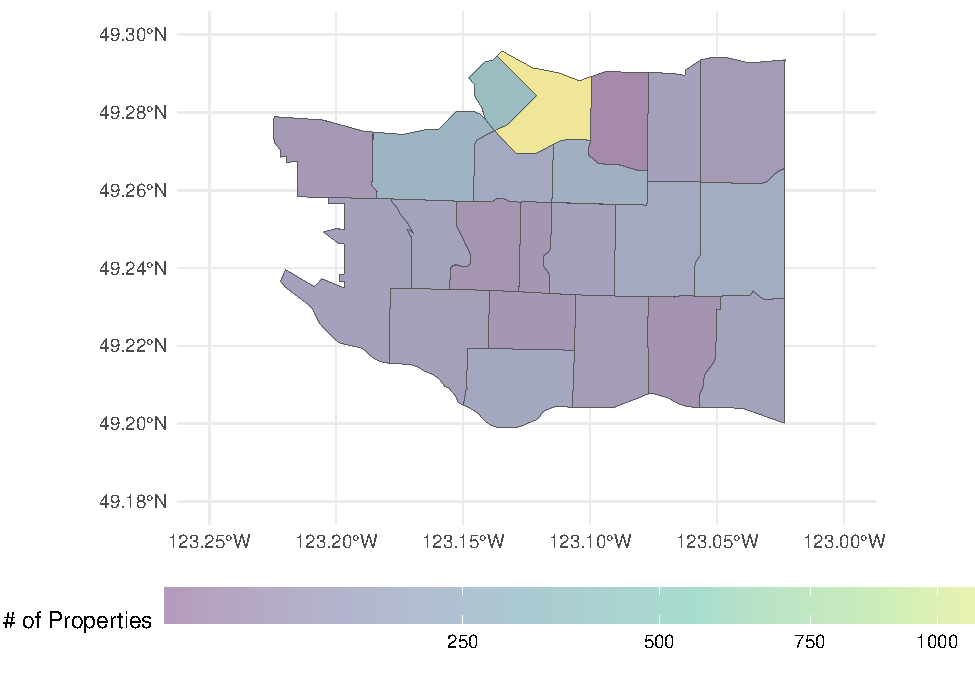
\includegraphics{final_report_files/figure-latex/unnamed-chunk-42-1.pdf}
\caption{Choropleth Map for the Number of Properties in Each
Neighbourhood}
\end{figure}

\begin{longtable}[]{@{}lr@{}}
\caption{Number of Properties in Each Vancouver
Neighborhood}\tabularnewline
\toprule()
Neighborhood & Number of Propereties \\
\midrule()
\endfirsthead
\toprule()
Neighborhood & Number of Propereties \\
\midrule()
\endhead
Downtown & 1249 \\
West End & 349 \\
Kitsilano & 274 \\
Mount Pleasant & 223 \\
Renfrew-Collingwood & 211 \\
Kensington-Cedar Cottage & 168 \\
Fairview & 166 \\
Marpole & 165 \\
Arbutus-Ridge & 127 \\
Killarney & 126 \\
Dunbar-Southlands & 120 \\
Riley Park & 120 \\
Grandview-Woodland & 112 \\
Kerrisdale & 104 \\
Sunset & 90 \\
Hastings-Sunrise & 86 \\
West Point Grey & 79 \\
Oakridge & 70 \\
South Cambie & 65 \\
Shaughnessy & 60 \\
Victoria-Fraserview & 57 \\
Strathcona & 35 \\
\bottomrule()
\end{longtable}

\begin{longtable}[]{@{}
  >{\raggedright\arraybackslash}p{(\columnwidth - 10\tabcolsep) * \real{0.3090}}
  >{\centering\arraybackslash}p{(\columnwidth - 10\tabcolsep) * \real{0.1348}}
  >{\centering\arraybackslash}p{(\columnwidth - 10\tabcolsep) * \real{0.1404}}
  >{\centering\arraybackslash}p{(\columnwidth - 10\tabcolsep) * \real{0.1404}}
  >{\centering\arraybackslash}p{(\columnwidth - 10\tabcolsep) * \real{0.1348}}
  >{\centering\arraybackslash}p{(\columnwidth - 10\tabcolsep) * \real{0.1404}}@{}}
\caption{Summary Statistics Housing Data}\tabularnewline
\toprule()
\begin{minipage}[b]{\linewidth}\raggedright
\end{minipage} & \begin{minipage}[b]{\linewidth}\centering
Apartment (N=2341)
\end{minipage} & \begin{minipage}[b]{\linewidth}\centering
Duplex (N=192)
\end{minipage} & \begin{minipage}[b]{\linewidth}\centering
House (N=1211)
\end{minipage} & \begin{minipage}[b]{\linewidth}\centering
Townhouse (N=312)
\end{minipage} & \begin{minipage}[b]{\linewidth}\centering
Total (N=4056)
\end{minipage} \\
\midrule()
\endfirsthead
\toprule()
\begin{minipage}[b]{\linewidth}\raggedright
\end{minipage} & \begin{minipage}[b]{\linewidth}\centering
Apartment (N=2341)
\end{minipage} & \begin{minipage}[b]{\linewidth}\centering
Duplex (N=192)
\end{minipage} & \begin{minipage}[b]{\linewidth}\centering
House (N=1211)
\end{minipage} & \begin{minipage}[b]{\linewidth}\centering
Townhouse (N=312)
\end{minipage} & \begin{minipage}[b]{\linewidth}\centering
Total (N=4056)
\end{minipage} \\
\midrule()
\endhead
\textbf{square\_feet} & & & & & \\
~~~Mean (SE) & 939.31 (10.30) & 1763.59 (47.50) & 2473.88 (42.63) &
1493.10 (26.60) & 1479.10 (17.94) \\
~~~Median & 820.00 & 1594.00 & 2300.00 & 1405.00 & 1079.50 \\
~~~Q1,Q3 & 623.00, 1105.00 & 1425.25, 1916.00 & 1222.00, 3434.00 &
1227.00, 1668.00 & 720.75, 1750.25 \\
~~~Range & 317.00 - 7136.00 & 900.00 - 5600.00 & 435.00 - 9347.00 &
528.00 - 4152.00 & 317.00 - 9347.00 \\
\textbf{price} & & & & & \\
~~~Mean (SE) & 1216199.59 (20610.19) & 2056666.88 (56438.74) &
2898611.11 (56439.62) & 1740670.80 (44697.60) & 1798646.60 (24132.55) \\
~~~Median & 875000.00 & 1788900.00 & 2388000.00 & 1599000.00 &
1269000.00 \\
~~~Q1,Q3 & 688000.00, 1350000.00 & 1521750.00, 2448000.00 & 1433500.00,
4188000.00 & 1275000.00, 1925000.00 & 779675.00, 2149000.00 \\
~~~Range & 215000.00 - 9988000.00 & 1112000.00 - 6000000.00 & 399000.00
- 10000000.00 & 599000.00 - 7890000.00 & 215000.00 - 10000000.00 \\
\textbf{beds} & & & & & \\
~~~Mean (SE) & 1.64 (0.02) & 3.79 (0.09) & 4.15 (0.06) & 2.60 (0.04) &
2.57 (0.03) \\
~~~Median & 2.00 & 3.00 & 4.00 & 3.00 & 2.00 \\
~~~Q1,Q3 & 1.00, 2.00 & 3.00, 4.00 & 2.00, 6.00 & 2.00, 3.00 & 1.00,
3.00 \\
~~~Range & 0.00 - 7.00 & 1.00 - 12.00 & 0.00 - 13.00 & 1.00 - 5.00 &
0.00 - 13.00 \\
\textbf{baths} & & & & & \\
~~~Mean (SE) & 1.61 (0.01) & 3.68 (0.09) & 3.32 (0.06) & 2.64 (0.04) &
2.30 (0.02) \\
~~~Median & 2.00 & 4.00 & 3.00 & 3.00 & 2.00 \\
~~~Q1,Q3 & 1.00, 2.00 & 3.00, 4.00 & 2.00, 4.00 & 2.00, 3.00 & 1.00,
3.00 \\
~~~Range & 0.00 - 8.00 & 2.00 - 11.00 & 0.00 - 11.00 & 1.00 - 5.00 &
0.00 - 11.00 \\
\textbf{lot\_size} & & & & & \\
~~~Mean (SE) & 0.00 (0.00) & 1962.24 (169.38) & 4050.23 (115.99) & 73.41
(48.37) & 1307.81 (45.91) \\
~~~Median & 0.00 & 0.00 & 4007.52 & 0.00 & 0.00 \\
~~~Q1,Q3 & 0.00, 0.00 & 0.00, 4026.00 & 0.00, 6145.00 & 0.00, 0.00 &
0.00, 0.00 \\
~~~Range & 0.00 - 0.00 & 0.00 - 8038.80 & 0.00 - 39770.28 & 0.00 -
10629.00 & 0.00 - 39770.28 \\
\textbf{neighborhood} & & & & & \\
~~~Arbutus-Ridge & 46 (2.0\%) & 3 (1.6\%) & 71 (5.9\%) & 7 (2.2\%) & 127
(3.1\%) \\
~~~Downtown & 1027 (43.9\%) & 1 (0.5\%) & 166 (13.7\%) & 55 (17.6\%) &
1249 (30.8\%) \\
~~~Dunbar-Southlands & 9 (0.4\%) & 8 (4.2\%) & 101 (8.3\%) & 2 (0.6\%) &
120 (3.0\%) \\
~~~Fairview & 106 (4.5\%) & 5 (2.6\%) & 35 (2.9\%) & 20 (6.4\%) & 166
(4.1\%) \\
~~~Grandview-Woodland & 43 (1.8\%) & 13 (6.8\%) & 48 (4.0\%) & 8 (2.6\%)
& 112 (2.8\%) \\
~~~Hastings-Sunrise & 16 (0.7\%) & 23 (12.0\%) & 45 (3.7\%) & 2 (0.6\%)
& 86 (2.1\%) \\
~~~Kensington-Cedar Cottage & 33 (1.4\%) & 35 (18.2\%) & 93 (7.7\%) & 7
(2.2\%) & 168 (4.1\%) \\
~~~Kerrisdale & 28 (1.2\%) & 4 (2.1\%) & 65 (5.4\%) & 7 (2.2\%) & 104
(2.6\%) \\
~~~Killarney & 76 (3.2\%) & 3 (1.6\%) & 26 (2.1\%) & 21 (6.7\%) & 126
(3.1\%) \\
~~~Kitsilano & 150 (6.4\%) & 19 (9.9\%) & 75 (6.2\%) & 30 (9.6\%) & 274
(6.8\%) \\
~~~Marpole & 82 (3.5\%) & 12 (6.2\%) & 51 (4.2\%) & 20 (6.4\%) & 165
(4.1\%) \\
~~~Mount Pleasant & 152 (6.5\%) & 8 (4.2\%) & 36 (3.0\%) & 27 (8.7\%) &
223 (5.5\%) \\
~~~Oakridge & 21 (0.9\%) & 2 (1.0\%) & 28 (2.3\%) & 19 (6.1\%) & 70
(1.7\%) \\
~~~Renfrew-Collingwood & 116 (5.0\%) & 18 (9.4\%) & 58 (4.8\%) & 19
(6.1\%) & 211 (5.2\%) \\
~~~Riley Park & 33 (1.4\%) & 4 (2.1\%) & 45 (3.7\%) & 38 (12.2\%) & 120
(3.0\%) \\
~~~Shaughnessy & 3 (0.1\%) & 0 (0.0\%) & 46 (3.8\%) & 11 (3.5\%) & 60
(1.5\%) \\
~~~South Cambie & 38 (1.6\%) & 0 (0.0\%) & 21 (1.7\%) & 6 (1.9\%) & 65
(1.6\%) \\
~~~Strathcona & 23 (1.0\%) & 1 (0.5\%) & 6 (0.5\%) & 5 (1.6\%) & 35
(0.9\%) \\
~~~Sunset & 19 (0.8\%) & 16 (8.3\%) & 55 (4.5\%) & 0 (0.0\%) & 90
(2.2\%) \\
~~~Victoria-Fraserview & 10 (0.4\%) & 10 (5.2\%) & 36 (3.0\%) & 1
(0.3\%) & 57 (1.4\%) \\
~~~West End & 294 (12.6\%) & 0 (0.0\%) & 50 (4.1\%) & 5 (1.6\%) & 349
(8.6\%) \\
~~~West Point Grey & 16 (0.7\%) & 7 (3.6\%) & 54 (4.5\%) & 2 (0.6\%) &
79 (1.9\%) \\
\textbf{lng} & & & & & \\
~~~Mean (SE) & -123.12 (0.00) & -123.10 (0.00) & -123.12 (0.00) &
-123.11 (0.00) & -123.12 (0.00) \\
~~~Median & -123.12 & -123.08 & -123.12 & -123.12 & -123.12 \\
~~~Q1,Q3 & -123.13, -123.11 & -123.13, -123.06 & -123.15, -123.08 &
-123.13, -123.10 & -123.14, -123.10 \\
~~~Range & -123.21 - -123.02 & -123.21 - -123.03 & -123.22 - -123.02 &
-123.21 - -123.03 & -123.22 - -123.02 \\
\textbf{lat} & & & & & \\
~~~Mean (SE) & 49.27 (0.00) & 49.25 (0.00) & 49.25 (0.00) & 49.25 (0.00)
& 49.26 (0.00) \\
~~~Median & 49.27 & 49.25 & 49.25 & 49.26 & 49.27 \\
~~~Q1,Q3 & 49.26, 49.28 & 49.23, 49.27 & 49.24, 49.27 & 49.24, 49.27 &
49.24, 49.28 \\
~~~Range & 49.20 - 49.29 & 49.21 - 49.29 & 49.20 - 49.29 & 49.20 - 49.29
& 49.20 - 49.29 \\
\textbf{sky\_train} & & & & & \\
~~~Mean (SE) & 1018.97 (21.06) & 2069.48 (102.89) & 2069.36 (47.37) &
1276.83 (62.27) & 1402.15 (21.29) \\
~~~Median & 636.24 & 1749.68 & 1668.76 & 880.11 & 816.77 \\
~~~Q1,Q3 & 381.35, 1271.19 & 1039.85, 2716.59 & 706.79, 3044.28 &
534.60, 1762.46 & 447.42, 1986.40 \\
~~~Range & 30.49 - 6846.76 & 185.97 - 6245.08 & 30.49 - 7081.98 & 40.91
- 6400.98 & 30.49 - 7081.98 \\
\textbf{bus\_stop} & & & & & \\
~~~Mean (SE) & 102.88 (1.43) & 146.41 (7.10) & 157.87 (3.43) & 135.58
(5.04) & 123.88 (1.47) \\
~~~Median & 87.37 & 129.31 & 122.19 & 112.20 & 96.91 \\
~~~Q1,Q3 & 55.08, 130.10 & 61.50, 217.16 & 75.33, 218.33 & 70.21, 179.71
& 62.11, 157.47 \\
~~~Range & 5.79 - 415.56 & 5.86 - 424.69 & 5.86 - 1029.29 & 10.79 -
641.30 & 5.79 - 1029.29 \\
\textbf{parks} & & & & & \\
~~~Mean (SE) & 240.62 (2.85) & 353.05 (12.59) & 349.40 (5.48) & 304.42
(8.62) & 283.33 (2.61) \\
~~~Median & 221.74 & 338.21 & 322.17 & 274.81 & 257.81 \\
~~~Q1,Q3 & 144.17, 311.01 & 212.47, 476.34 & 202.96, 473.04 & 191.59,
406.53 & 156.46, 360.52 \\
~~~Range & 14.77 - 817.17 & 31.20 - 855.86 & 12.51 - 1004.66 & 13.31 -
738.60 & 12.51 - 1004.66 \\
\textbf{schools} & & & & & \\
~~~Mean (SE) & 394.93 (4.44) & 345.79 (10.85) & 388.95 (5.78) & 364.33
(10.96) & 388.47 (3.25) \\
~~~Median & 375.11 & 324.97 & 359.33 & 346.16 & 364.04 \\
~~~Q1,Q3 & 240.29, 509.24 & 236.98, 450.93 & 242.23, 494.20 & 240.40,
452.95 & 239.68, 494.35 \\
~~~Range & 4.10 - 1222.16 & 46.59 - 953.07 & 12.91 - 1177.76 & 52.33 -
1286.84 & 4.10 - 1286.84 \\
\textbf{commercial\_services} & & & & & \\
~~~Mean (SE) & 100.32 (1.50) & 39.49 (3.10) & 53.70 (1.73) & 77.90
(3.81) & 81.79 (1.12) \\
~~~Median & 87.00 & 29.00 & 39.00 & 78.00 & 66.00 \\
~~~Q1,Q3 & 47.00, 154.00 & 0.00, 69.50 & 0.00, 86.00 & 12.00, 110.50 &
25.00, 124.00 \\
~~~Range & 0.00 - 309.00 & 0.00 - 155.00 & 0.00 - 309.00 & 0.00 - 297.00
& 0.00 - 309.00 \\
\textbf{food\_beverages} & & & & & \\
~~~Mean (SE) & 132.56 (2.20) & 27.65 (2.79) & 56.13 (2.44) & 73.38
(5.08) & 100.22 (1.64) \\
~~~Median & 118.00 & 15.00 & 19.00 & 55.00 & 61.00 \\
~~~Q1,Q3 & 38.00, 203.00 & 0.00, 42.00 & 0.00, 70.00 & 8.00, 104.00 &
14.00, 160.00 \\
~~~Range & 0.00 - 450.00 & 0.00 - 322.00 & 0.00 - 448.00 & 0.00 - 428.00
& 0.00 - 450.00 \\
\textbf{website} & & & & & \\
~~~point2home & 491 (21.0\%) & 0 (0.0\%) & 483 (39.9\%) & 0 (0.0\%) &
974 (24.0\%) \\
~~~remax & 1376 (58.8\%) & 7 (3.6\%) & 0 (0.0\%) & 125 (40.1\%) & 1508
(37.2\%) \\
~~~rew & 474 (20.2\%) & 63 (32.8\%) & 161 (13.3\%) & 68 (21.8\%) & 766
(18.9\%) \\
~~~zolo & 0 (0.0\%) & 122 (63.5\%) & 567 (46.8\%) & 119 (38.1\%) & 808
(19.9\%) \\
\textbf{break\_and\_enter\_commercial} & & & & & \\
~~~Mean (SE) & 310.27 (4.67) & 63.11 (4.44) & 130.49 (5.16) & 159.83
(10.93) & 233.32 (3.53) \\
~~~Median & 219.00 & 49.00 & 49.00 & 97.00 & 144.00 \\
~~~Q1,Q3 & 97.00, 558.00 & 16.00, 87.00 & 16.00, 144.00 & 26.00, 188.00
& 40.00, 558.00 \\
~~~Range & 2.00 - 558.00 & 2.00 - 558.00 & 2.00 - 558.00 & 2.00 - 558.00
& 2.00 - 558.00 \\
\textbf{break\_and\_enter\_residential\_other} & & & & & \\
~~~Mean (SE) & 75.64 (0.58) & 62.27 (2.22) & 58.97 (0.88) & 69.33 (1.93)
& 69.54 (0.48) \\
~~~Median & 86.00 & 59.00 & 59.00 & 84.00 & 84.00 \\
~~~Q1,Q3 & 45.00, 86.00 & 31.00, 84.00 & 31.00, 86.00 & 39.00, 86.00 &
42.00, 86.00 \\
~~~Range & 9.00 - 121.00 & 9.00 - 121.00 & 9.00 - 121.00 & 9.00 - 121.00
& 9.00 - 121.00 \\
\textbf{mischief} & & & & & \\
~~~Mean (SE) & 931.55 (15.83) & 181.02 (12.23) & 384.23 (16.51) & 462.61
(35.49) & 696.54 (11.61) \\
~~~Median & 466.00 & 175.00 & 175.00 & 202.00 & 303.00 \\
~~~Q1,Q3 & 254.00, 1787.00 & 74.00, 202.00 & 51.00, 366.00 & 62.00,
366.00 & 105.00, 1787.00 \\
~~~Range & 20.00 - 1787.00 & 20.00 - 1787.00 & 20.00 - 1787.00 & 20.00 -
1787.00 & 20.00 - 1787.00 \\
\textbf{other\_theft} & & & & & \\
~~~Mean (SE) & 1555.08 (23.81) & 421.64 (31.05) & 700.94 (26.20) &
828.95 (55.77) & 1190.55 (17.79) \\
~~~Median & 990.00 & 277.00 & 277.00 & 309.00 & 832.00 \\
~~~Q1,Q3 & 602.00, 2816.00 & 67.00, 639.00 & 78.00, 862.00 & 115.00,
990.00 & 227.00, 2816.00 \\
~~~Range & 15.00 - 2816.00 & 15.00 - 2816.00 & 15.00 - 2816.00 & 15.00 -
2816.00 & 15.00 - 2816.00 \\
\textbf{theft\_from\_vehicle} & & & & & \\
~~~Mean (SE) & 1216.73 (20.33) & 276.93 (14.37) & 511.90 (21.15) &
612.19 (45.57) & 915.30 (14.89) \\
~~~Median & 566.00 & 295.00 & 256.00 & 256.00 & 412.00 \\
~~~Q1,Q3 & 412.00, 2319.00 & 148.00, 358.00 & 83.00, 412.00 & 97.00,
479.00 & 211.00, 2319.00 \\
~~~Range & 20.00 - 2319.00 & 20.00 - 2319.00 & 20.00 - 2319.00 & 20.00 -
2319.00 & 20.00 - 2319.00 \\
\textbf{theft\_of\_bicycle} & & & & & \\
~~~Mean (SE) & 214.29 (2.75) & 51.81 (3.94) & 93.60 (3.35) & 119.10
(7.04) & 163.25 (2.18) \\
~~~Median & 202.00 & 46.00 & 43.00 & 51.00 & 123.00 \\
~~~Q1,Q3 & 72.00, 348.00 & 13.00, 51.00 & 13.00, 123.00 & 16.00, 202.00
& 28.00, 348.00 \\
~~~Range & 2.00 - 348.00 & 2.00 - 348.00 & 2.00 - 348.00 & 2.00 - 348.00
& 2.00 - 348.00 \\
\textbf{theft\_of\_vehicle} & & & & & \\
~~~Mean (SE) & 70.26 (0.56) & 49.58 (1.80) & 46.20 (0.89) & 50.50 (1.72)
& 60.58 (0.48) \\
~~~Median & 75.00 & 62.00 & 43.00 & 43.00 & 64.00 \\
~~~Q1,Q3 & 53.00, 96.00 & 30.00, 73.00 & 14.00, 73.00 & 20.00, 75.00 &
39.50, 96.00 \\
~~~Range & 3.00 - 96.00 & 3.00 - 96.00 & 3.00 - 96.00 & 3.00 - 96.00 &
3.00 - 96.00 \\
\textbf{vehicle\_collision\_or\_pedestrian\_struck\_with\_injury} & & &
& & \\
~~~Mean (SE) & 94.36 (1.09) & 52.42 (1.55) & 55.33 (1.27) & 61.20 (2.57)
& 78.17 (0.82) \\
~~~Median & 65.00 & 54.00 & 45.00 & 45.00 & 60.00 \\
~~~Q1,Q3 & 51.00, 152.00 & 45.00, 71.00 & 13.00, 71.00 & 27.00, 65.00 &
45.00, 152.00 \\
~~~Range & 9.00 - 152.00 & 9.00 - 152.00 & 9.00 - 152.00 & 9.00 - 152.00
& 9.00 - 152.00 \\
\bottomrule()
\end{longtable}

\begin{figure}
\centering
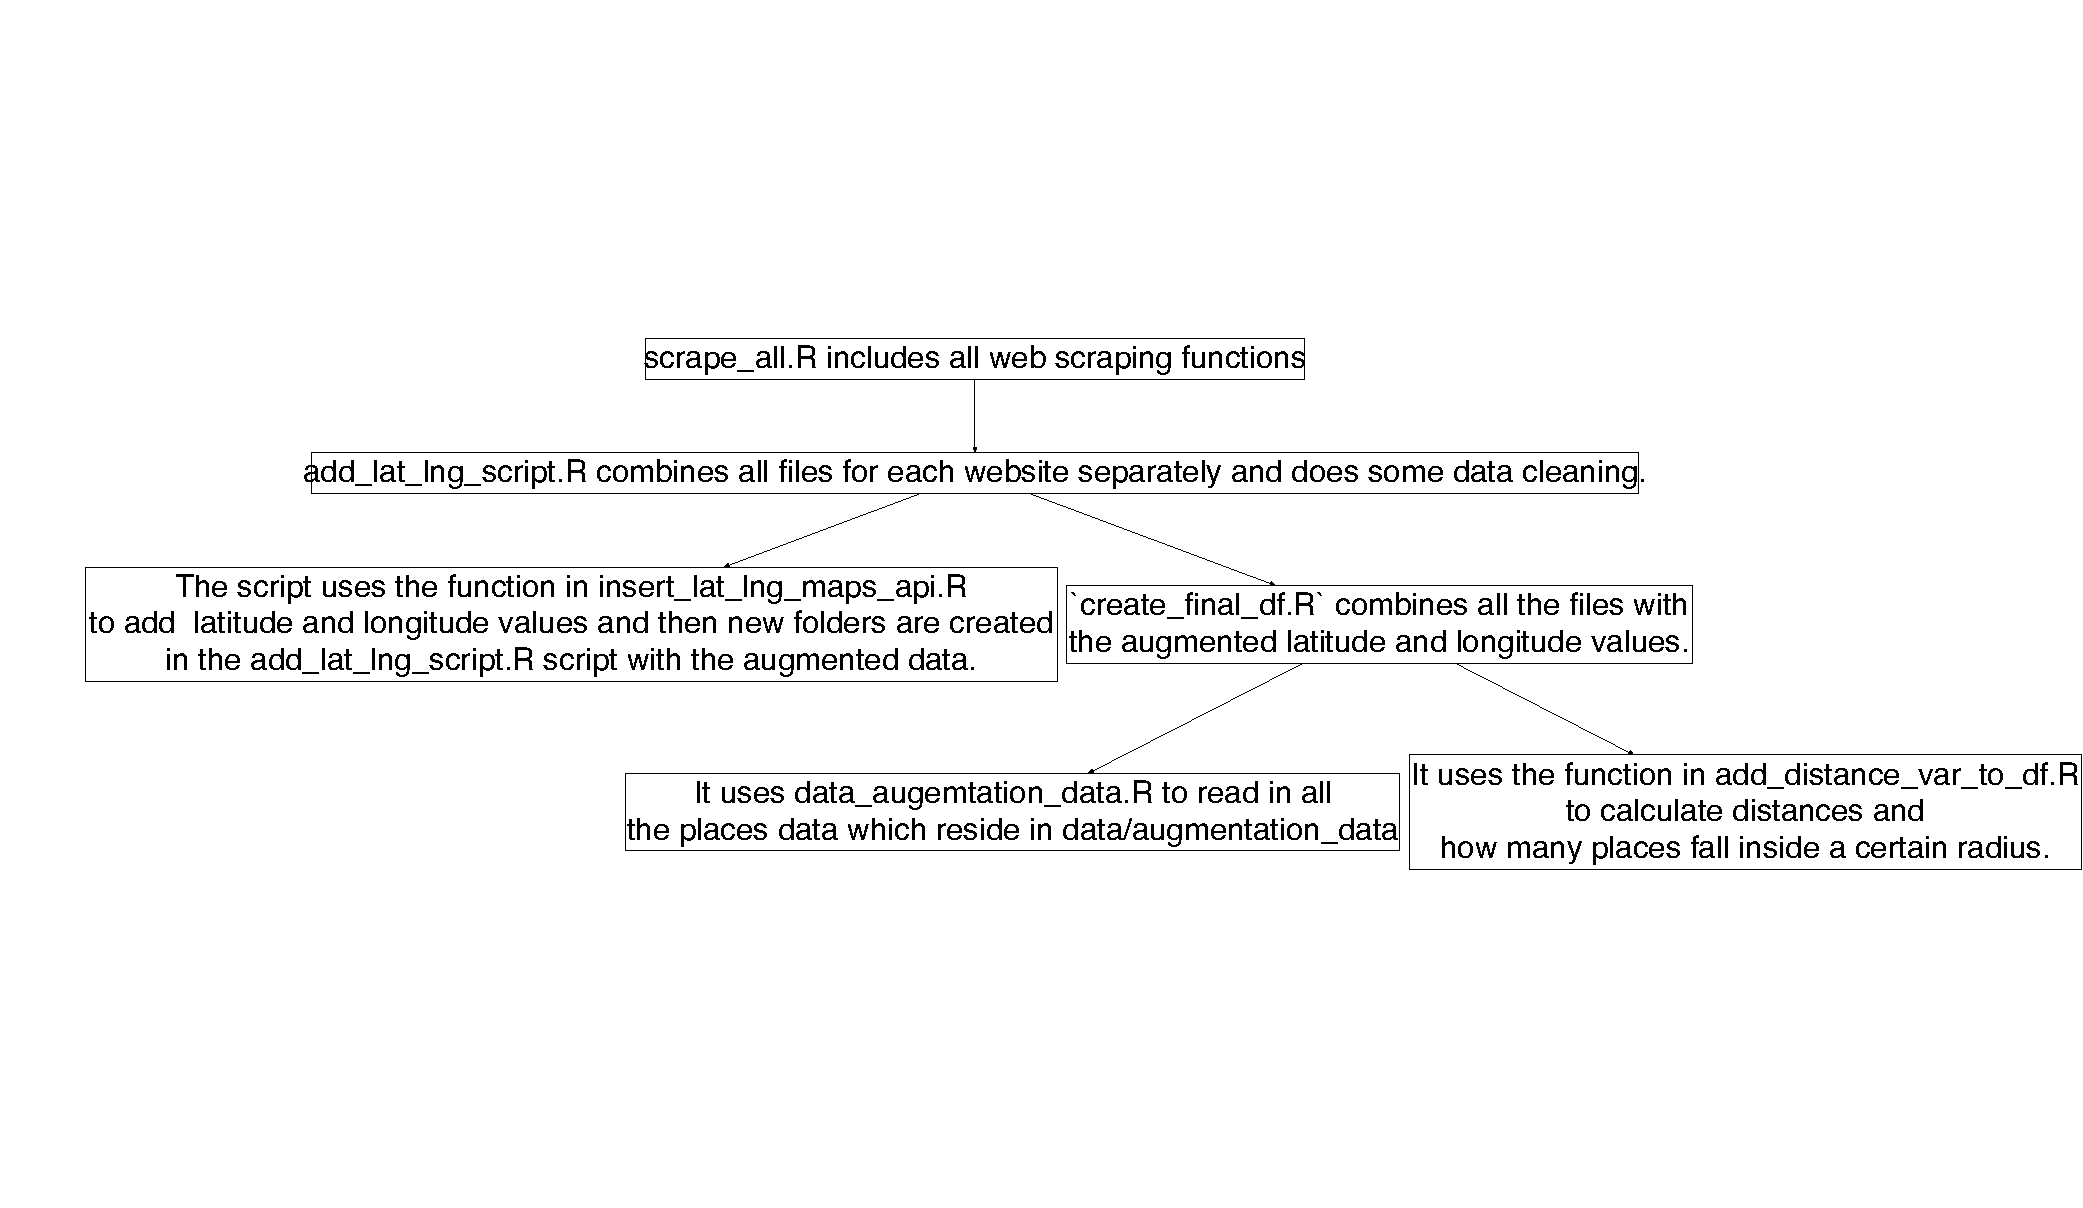
\includegraphics{final_report_files/figure-latex/unnamed-chunk-45-1.pdf}
\caption{R Functions and Scripts to Create the Final Data Set}
\end{figure}

\end{document}
